%% bare_jrnl.tex
%% V1.4
%% 2012/12/27
%% by Michael Shell
%% see http://www.michaelshell.org/
%% for current contact information.
%%
%% This is a skeleton file demonstrating the use of IEEEtran.cls
%% (requires IEEEtran.cls version 1.8 or later) with an IEEE journal paper.
%%
%% Support sites:
%% http://www.michaelshell.org/tex/ieeetran/
%% http://www.ctan.org/tex-archive/macros/latex/contrib/IEEEtran/
%% and
%% http://www.ieee.org/



% *** Authors should verify (and, if needed, correct) their LaTeX system  ***
% *** with the testflow diagnostic prior to trusting their LaTeX platform ***
% *** with production work. IEEE's font choices can trigger bugs that do  ***
% *** not appear when using other class files.                            ***
% The testflow support page is at:
% http://www.michaelshell.org/tex/testflow/


%%*************************************************************************
%% Legal Notice:
%% This code is offered as-is without any warranty either expressed or
%% implied; without even the implied warranty of MERCHANTABILITY or
%% FITNESS FOR A PARTICULAR PURPOSE!
%% User assumes all risk.
%% In no event shall IEEE or any contributor to this code be liable for
%% any damages or losses, including, but not limited to, incidental,
%% consequential, or any other damages, resulting from the use or misuse
%% of any information contained here.
%%
%% All comments are the opinions of their respective authors and are not
%% necessarily endorsed by the IEEE.
%%
%% This work is distributed under the LaTeX Project Public License (LPPL)
%% ( http://www.latex-project.org/ ) version 1.3, and may be freely used,
%% distributed and modified. A copy of the LPPL, version 1.3, is included
%% in the base LaTeX documentation of all distributions of LaTeX released
%% 2003/12/01 or later.
%% Retain all contribution notices and credits.
%% ** Modified files should be clearly indicated as such, including  **
%% ** renaming them and changing author support contact information. **
%%
%% File list of work: IEEEtran.cls, IEEEtran_HOWTO.pdf, bare_adv.tex,
%%                    bare_conf.tex, bare_jrnl.tex, bare_jrnl_compsoc.tex,
%%                    bare_jrnl_transmag.tex
%%*************************************************************************

% Note that the a4paper option is mainly intended so that authors in
% countries using A4 can easily print to A4 and see how their papers will
% look in print - the typesetting of the document will not typically be
% affected with changes in paper size (but the bottom and side margins will).
% Use the testflow package mentioned above to verify correct handling of
% both paper sizes by the user's LaTeX system.
%
% Also note that the "draftcls" or "draftclsnofoot", not "draft", option
% should be used if it is desired that the figures are to be displayed in
% draft mode.
%
\documentclass[journal,UTF8]{IEEEtran}
\usepackage{color}
%
% If IEEEtran.cls has not been installed into the LaTeX system files,
% manually specify the path to it like:
%\documentclass[journal]{../sty/IEEEtran}





% Some very useful LaTeX packages include:
% (uncomment the ones you want to load)


% *** MISC UTILITY PACKAGES ***
%
%\usepackage{ifpdf}
% Heiko Oberdiek's ifpdf.sty is very useful if you need conditional
% compilation based on whether the output is pdf or dvi.
% usage:
% \ifpdf
%   % pdf code
% \else
%   % dvi code
% \fi
% The latest version of ifpdf.sty can be obtained from:
% http://www.ctan.org/tex-archive/macros/latex/contrib/oberdiek/
% Also, note that IEEEtran.cls V1.7 and later provides a builtin
% \ifCLASSINFOpdf conditional that works the same way.
% When switching from latex to pdflatex and vice-versa, the compiler may
% have to be run twice to clear warning/error messages.






% *** CITATION PACKAGES ***
%
\usepackage{cite}
% cite.sty was written by Donald Arseneau
% V1.6 and later of IEEEtran pre-defines the format of the cite.sty package
% \cite{} output to follow that of IEEE. Loading the cite package will
% result in citation numbers being automatically sorted and properly
% "compressed/ranged". e.g., [1], [9], [2], [7], [5], [6] without using
% cite.sty will become [1], [2], [5]--[7], [9] using cite.sty. cite.sty's
% \cite will automatically add leading space, if needed. Use cite.sty's
% noadjust option (cite.sty V3.8 and later) if you want to turn this off
% such as if a citation ever needs to be enclosed in parenthesis.
% cite.sty is already installed on most LaTeX systems. Be sure and use
% version 4.0 (2003-05-27) and later if using hyperref.sty. cite.sty does
% not currently provide for hyperlinked citations.
% The latest version can be obtained at:
% http://www.ctan.org/tex-archive/macros/latex/contrib/cite/
% The documentation is contained in the cite.sty file itself.






% *** GRAPHICS RELATED PACKAGES ***
%
\ifCLASSINFOpdf
 \usepackage[pdftex]{graphicx}
  % declare the path(s) where your graphic files are
 \graphicspath{{../pdf/}{../jpeg/}}
  % and their extensions so you won't have to specify these with
  % every instance of \includegraphics
\DeclareGraphicsExtensions{.pdf,.jpeg,.png}
\else
  % or other class option (dvipsone, dvipdf, if not using dvips). graphicx
  % will default to the driver specified in the system graphics.cfg if no
  % driver is specified.
\usepackage[dvips]{graphicx}
  % declare the path(s) where your graphic files are
\graphicspath{{../eps/}}
  % and their extensions so you won't have to specify these with
  % every instance of \includegraphics
\DeclareGraphicsExtensions{.eps}
\fi
% graphicx was written by David Carlisle and Sebastian Rahtz. It is
% required if you want graphics, photos, etc. graphicx.sty is already
% installed on most LaTeX systems. The latest version and documentation
% can be obtained at:
% http://www.ctan.org/tex-archive/macros/latex/required/graphics/
% Another good source of documentation is "Using Imported Graphics in
% LaTeX2e" by Keith Reckdahl which can be found at:
% http://www.ctan.org/tex-archive/info/epslatex/
%
% latex, and pdflatex in dvi mode, support graphics in encapsulated
% postscript (.eps) format. pdflatex in pdf mode supports graphics
% in .pdf, .jpeg, .png and .mps (metapost) formats. Users should ensure
% that all non-photo figures use a vector format (.eps, .pdf, .mps) and
% not a bitmapped formats (.jpeg, .png). IEEE frowns on bitmapped formats
% which can result in "jaggedy"/blurry rendering of lines and letters as
% well as large increases in file sizes.
%
% You can find documentation about the pdfTeX application at:
% http://www.tug.org/applications/pdftex





% *** MATH PACKAGES ***
%
\usepackage[cmex10]{amsmath}
% A popular package from the American Mathematical Society that provides
% many useful and powerful commands for dealing with mathematics. If using
% it, be sure to load this package with the cmex10 option to ensure that
% only type 1 fonts will utilized at all point sizes. Without this option,
% it is possible that some math symbols, particularly those within
% footnotes, will be rendered in bitmap form which will result in a
% document that can not be IEEE Xplore compliant!
%
% Also, note that the amsmath package sets \interdisplaylinepenalty to 10000
% thus preventing page breaks from occurring within multiline equations. Use:
%\interdisplaylinepenalty=2500
% after loading amsmath to restore such page breaks as IEEEtran.cls normally
% does. amsmath.sty is already installed on most LaTeX systems. The latest
% version and documentation can be obtained at:
% http://www.ctan.org/tex-archive/macros/latex/required/amslatex/math/





% *** SPECIALIZED LIST PACKAGES ***
%
%\usepackage{algorithmic}
\usepackage[ruled]{algorithm2e}
% algorithmic.sty was written by Peter Williams and Rogerio Brito.
% This package provides an algorithmic environment fo describing algorithms.
% You can use the algorithmic environment in-text or within a figure
% environment to provide for a floating algorithm. Do NOT use the algorithm
% floating environment provided by algorithm.sty (by the same authors) or
% algorithm2e.sty (by Christophe Fiorio) as IEEE does not use dedicated
% algorithm float types and packages that provide these will not provide
% correct IEEE style captions. The latest version and documentation of
% algorithmic.sty can be obtained at:
% http://www.ctan.org/tex-archive/macros/latex/contrib/algorithms/
% There is also a support site at:
% http://algorithms.berlios.de/index.html
% Also of interest may be the (relatively newer and more customizable)
% algorithmicx.sty package by Szasz Janos:
% http://www.ctan.org/tex-archive/macros/latex/contrib/algorithmicx/




% *** ALIGNMENT PACKAGES ***
%
\usepackage{array}

% Frank Mittelbach's and David Carlisle's array.sty patches and improves
% the standard LaTeX2e array and tabular environments to provide better
% appearance and additional user controls. As the default LaTeX2e table
% generation code is lacking to the point of almost being broken with
% respect to the quality of the end results, all users are strongly
% advised to use an enhanced (at the very least that provided by array.sty)
% set of table tools. array.sty is already installed on most systems. The
% latest version and documentation can be obtained at:
% http://www.ctan.org/tex-archive/macros/latex/required/tools/


% IEEEtran contains the IEEEeqnarray family of commands that can be used to
% generate multiline equations as well as matrices, tables, etc., of high
% quality.




% *** SUBFIGURE PACKAGES ***
\ifCLASSOPTIONcompsoc
  \usepackage[caption=false,font=normalsize,labelfont=sf,textfont=sf]{subfig}
\else
  \usepackage[caption=false,font=footnotesize]{subfig}
\fi
% subfig.sty, written by Steven Douglas Cochran, is the modern replacement
% for subfigure.sty, the latter of which is no longer maintained and is
% incompatible with some LaTeX packages including fixltx2e. However,
% subfig.sty requires and automatically loads Axel Sommerfeldt's caption.sty
% which will override IEEEtran.cls' handling of captions and this will result
% in non-IEEE style figure/table captions. To prevent this problem, be sure
% and invoke subfig.sty's "caption=false" package option (available since
% subfig.sty version 1.3, 2005/06/28) as this is will preserve IEEEtran.cls
% handling of captions.
% Note that the Computer Society format requires a larger sans serif font
% than the serif footnote size font used in traditional IEEE formatting
% and thus the need to invoke different subfig.sty package options depending
% on whether compsoc mode has been enabled.
%
% The latest version and documentation of subfig.sty can be obtained at:
% http://www.ctan.org/tex-archive/macros/latex/contrib/subfig/




% *** FLOAT PACKAGES ***
%
%\usepackage{fixltx2e}
% fixltx2e, the successor to the earlier fix2col.sty, was written by
% Frank Mittelbach and David Carlisle. This package corrects a few problems
% in the LaTeX2e kernel, the most notable of which is that in current
% LaTeX2e releases, the ordering of single and double column floats is not
% guaranteed to be preserved. Thus, an unpatched LaTeX2e can allow a
% single column figure to be placed prior to an earlier double column
% figure. The latest version and documentation can be found at:
% http://www.ctan.org/tex-archive/macros/latex/base/


%\usepackage{stfloats}
% stfloats.sty was written by Sigitas Tolusis. This package gives LaTeX2e
% the ability to do double column floats at the bottom of the page as well
% as the top. (e.g., "\begin{figure*}[!b]" is not normally possible in
% LaTeX2e). It also provides a command:
%\fnbelowfloat
% to enable the placement of footnotes below bottom floats (the standard
% LaTeX2e kernel puts them above bottom floats). This is an invasive package
% which rewrites many portions of the LaTeX2e float routines. It may not work
% with other packages that modify the LaTeX2e float routines. The latest
% version and documentation can be obtained at:
% http://www.ctan.org/tex-archive/macros/latex/contrib/sttools/
% Do not use the stfloats baselinefloat ability as IEEE does not allow
% \baselineskip to stretch. Authors submitting work to the IEEE should note
% that IEEE rarely uses double column equations and that authors should try
% to avoid such use. Do not be tempted to use the cuted.sty or midfloat.sty
% packages (also by Sigitas Tolusis) as IEEE does not format its papers in
% such ways.
% Do not attempt to use stfloats with fixltx2e as they are incompatible.
% Instead, use Morten Hogholm'a dblfloatfix which combines the features
% of both fixltx2e and stfloats:
%
% \usepackage{dblfloatfix}
% The latest version can be found at:
% http://www.ctan.org/tex-archive/macros/latex/contrib/dblfloatfix/




%\ifCLASSOPTIONcaptionsoff
%  \usepackage[nomarkers]{endfloat}
% \let\MYoriglatexcaption\caption
% \renewcommand{\caption}[2][\relax]{\MYoriglatexcaption[#2]{#2}}
%\fi
% endfloat.sty was written by James Darrell McCauley, Jeff Goldberg and
% Axel Sommerfeldt. This package may be useful when used in conjunction with
% IEEEtran.cls'  captionsoff option. Some IEEE journals/societies require that
% submissions have lists of figures/tables at the end of the paper and that
% figures/tables without any captions are placed on a page by themselves at
% the end of the document. If needed, the draftcls IEEEtran class option or
% \CLASSINPUTbaselinestretch interface can be used to increase the line
% spacing as well. Be sure and use the nomarkers option of endfloat to
% prevent endfloat from "marking" where the figures would have been placed
% in the text. The two hack lines of code above are a slight modification of
% that suggested by in the endfloat docs (section 8.4.1) to ensure that
% the full captions always appear in the list of figures/tables - even if
% the user used the short optional argument of \caption[]{}.
% IEEE papers do not typically make use of \caption[]'s optional argument,
% so this should not be an issue. A similar trick can be used to disable
% captions of packages such as subfig.sty that lack options to turn off
% the subcaptions:
% For subfig.sty:
% \let\MYorigsubfloat\subfloat
% \renewcommand{\subfloat}[2][\relax]{\MYorigsubfloat[]{#2}}
% However, the above trick will not work if both optional arguments of
% the \subfloat command are used. Furthermore, there needs to be a
% description of each subfigure *somewhere* and endfloat does not add
% subfigure captions to its list of figures. Thus, the best approach is to
% avoid the use of subfigure captions (many IEEE journals avoid them anyway)
% and instead reference/explain all the subfigures within the main caption.
% The latest version of endfloat.sty and its documentation can obtained at:
% http://www.ctan.org/tex-archive/macros/latex/contrib/endfloat/
%
% The IEEEtran \ifCLASSOPTIONcaptionsoff conditional can also be used
% later in the document, say, to conditionally put the References on a
% page by themselves.




% *** PDF, URL AND HYPERLINK PACKAGES ***
%
%\usepackage{url}
% url.sty was written by Donald Arseneau. It provides better support for
% handling and breaking URLs. url.sty is already installed on most LaTeX
% systems. The latest version and documentation can be obtained at:
% http://www.ctan.org/tex-archive/macros/latex/contrib/url/
% Basically, \url{my_url_here}.




% *** Do not adjust lengths that control margins, column widths, etc. ***
% *** Do not use packages that alter fonts (such as pslatex).         ***
% There should be no need to do such things with IEEEtran.cls V1.6 and later.
% (Unless specifically asked to do so by the journal or conference you plan
% to submit to, of course. )


% correct bad hyphenation here
\hyphenation{op-tical net-works semi-conduc-tor}



\begin{document}
%
% paper title
% can use linebreaks \\ within to get better formatting as desired
% Do not put math or special symbols in the title.
\title{A User-oriented Development Method in \textcolor{red}{FSM supported} Multiprocessor Embeded PLCs}
%
%
% author names and IEEE memberships
% note positions of commas and nonbreaking spaces ( ~ ) LaTeX will not break
% a structure at a ~ so this keeps an author's name from being broken across
% two lines.
% use \thanks{} to gain access to the first footnote area
% a separate \thanks must be used for each paragraph as LaTeX2e's \thanks
% was not built to handle multiple paragraphs
%

%\author{Huifeng Wu,
%        Yi Yan, Danfeng Sun, Rene Simon% <-this % stops a space
%\thanks{Huifeng Wu and Yi Yan are with the Institute of Intelligent and Software Technology, Hangzhou Dianzi University, Hangzhou, 310018, China (e-mail: yybjyyj@163.com).}% <-this % stops a space
%\thanks{Danfeng Sun are with the Institute of Industrial Internet, Hangzhou Dianzi University, Hangzhou, 310018, China.}
%\thanks{Rene Simon is with the Department of Automation and Computer Sciences, Harz University of Applied Sciences, Wernigerode, 38855, Germany.}
%\thanks{This work was supported by a Grant from The National Natural Science Foundation of China(No.U1609211), Science and Technology Program of Zhejiang Province(No.2018C04001)}
%}% <-this % stops a space
%\thanks{Manuscript received April 19, 2005; revised December 27, 2012.}}

% note the % following the last \IEEEmembership and also \thanks -
% these prevent an unwanted space from occurring between the last author name
% and the end of the author line. i.e., if you had this:
%
% \author{....lastname \thanks{...} \thanks{...} }
%                     ^------------^------------^----Do not want these spaces!
%
% a space would be appended to the last name and could cause every name on that
% line to be shifted left slightly. This is one of those "LaTeX things". For
% instance, "\textbf{A} \textbf{B}" will typeset as "A B" not "AB". To get
% "AB" then you have to do: "\textbf{A}\textbf{B}"
% \thanks is no different in this regard, so shield the last } of each \thanks
% that ends a line with a % and do not let a space in before the next \thanks.
% Spaces after \IEEEmembership other than the last one are OK (and needed) as
% you are supposed to have spaces between the names. For what it is worth,
% this is a minor point as most people would not even notice if the said evil
% space somehow managed to creep in.



% The paper headers

%\markboth{Journal of \LaTeX\ Class Files,~Vol.~11, No.~4, December~2012}%
%{Shell \MakeLowercase{\textit{et al.}}: Bare Demo of IEEEtran.cls for Journals}

% The only time the second header will appear is for the odd numbered pages
% after the title page when using the twoside option.
%
% *** Note that you probably will NOT want to include the author's ***
% *** name in the headers of peer review papers.                   ***
% You can use \ifCLASSOPTIONpeerreview for conditional compilation here if
% you desire.




% If you want to put a publisher's ID mark on the page you can do it like
% this:
%\IEEEpubid{0000--0000/00\$00.00~\copyright~2012 IEEE}
% Remember, if you use this you must call \IEEEpubidadjcol in the second
% column for its text to clear the IEEEpubid mark.



% use for special paper notices
%\IEEEspecialpapernotice{(Invited Paper)}




% make the title area
\maketitle

% As a general rule, do not put math, special symbols or citations
% in the abstract or keywords.
% * <karyns@accdon.com> 2017-12-24T08:35:37.488Z:
% 

\begin{abstract}
  Programmable logic controllers ($PLC$s) are a base in automation, however applications become complex on logic and motion control mixed scenarios while the PC-based $PLC$ has high price and complex system which can not meet the customized requirement of large equipments. The development of $PLC$ has encountered bottlenecks. Hence, this paper presents a user-oriented development method. We pose a customized mulitprocessor $ePLC$ to enhance the performance, a multi-language supported uniform development platform to improve the adaptability of developers, an optimized system structure (reasonable memory allocation, user-oriented thread structure, proposed $LPM$ data interaction, modular software design, finite state machines) to reduce the development complexity. Ultimately, we adopt the proposed method to implement the distributed control system on a 200 ton injection molding machine. By comparison with TECHMATION and KEBA system, the startup time of the implemented system has been increased by more than 20 times while the key performance is almost identical. In addition, the implemented system adopts the customized multiprocessor $ePLC$ and detached human machine interface ($HMI$).
 
% * <karyns@accdon.com> 2017-12-24T08:32:14.912Z:
% 
% > customizable application layer
% Original wording was weird. Please confirm  change.
% 
% ^.
% * <karyns@accdon.com> 2017-12-24T08:28:06.592Z:
% 
% > changeable applications
% Meaning is unclear. Do you mean  "applications with multiple functions" or "different applications"? Please reword/clarify. 
% 
% ^.
% * <karyns@accdon.com> 2017-12-24T08:27:24.430Z:
% 
% > PLCs
% Please define.
% 
% ^.
\end{abstract}

% Note that keywords are not normally used for peerreview papers.
\begin{IEEEkeywords}
Multiprocessor, motion control, Injection Molding Machine, embedded PLC, User-oriented
\end{IEEEkeywords}

% For peer review papers, you can put extra information on the cover
% page as needed:
% \ifCLASSOPTIONpeerreview
% \begin{center} \bfseries EDICS Category: 3-BBND \end{center}
% \fi
%
% For peerreview papers, this IEEEtran command inserts a page break and
% creates the second title. It will be ignored for other modes.
\IEEEpeerreviewmaketitle



\section{Introduction}
Some concepts, such as smart factory, intelligent manufacturing \cite{Gonzalez2017Supervisory,Chekired2018Industrial}, and some technologies, such as Internet of Things, 5G, augment reality \cite{Li2018Energy,Ling20185G} are paving the road of the fourth industrial revolution. Normally, a typical plant is full of large equipments, for instance, cranes, CNC machining centers, injection molding machines ($IMM$s), air pumps, chillers, automatic guided vehicles and types of robots and most of them are controlled by the $PLC$. $PLC$s have become the main control system. Numerous researchers are focusing on $PLC$ technologies which extremely extends its application fields. \cite{Jiang2013System,Jiang2013Bayesian,Adiego2015Applying} guarantee the reliability by verifying the program of $PLC$s, \cite{Gerk2006Advanced,Chang2007Adaptive,Dominic2016PLC} improve the performance of $PLC$s using advanced algorithms, \cite{WuA} alleviates the development complexity of $PLC$s with a special software structure, \cite{Sch2013Development,Morenas2017Shop} pose methods to update $PLC$ programs dynamically.
However, with the rapidly ever-growing demands and the tend of applications to be user-oriented and complex logic and motion control mixed \cite{Zaeh2005A,Hossain2014Advanced}, $PLC$s still encountered bottlenecks, specially on large equipments (CNC machining center, $IMM$, etc.).

\subsection{Motivations}
To date, the hardware architecture of $PLC$s has two directions: $ePLC$s (embedded $PLC$s) and PC-based $PLC$s. PC-based $PLC$s are increasingly used on the applications of complex logic and motion control mixed scenarios on account of its high performance and lots of user-oriented tools \cite{Hossain2014Advanced}. Considering the IMM industry, Table \ref{table:IMMSystem} lists the composition of IMM, including parts(described as modules for programming), DI$\backslash$Os and AI$\backslash$Os. Normally, a simplest IMM system consists of 10 modules, 20 DIs, 30 DOs, 3 AIS and 7 AOs. Complex relations among them and high performance requirement of algorithms tremendously increase the difficulty of programming. Hence, as listed in Table \ref{table:IMMControllor}, the comparison of KEBA, BECKHOFF, GAFRAN and TECKMATION system which are the main brand of IMM controller illustrates that almost all of them are using PC-based PLCs. According to the complexity of the $IMM$ system and the software architecture of PC-based $PLC$, the $HMI$ is banded to $PLC$ which leads to little independence of $IMM$ manufacturers. 

$ePLC$s have a wide area of applications in automation due to its easy programming and high reliability, however some disadvantages still limit its further development \cite{Hossain2014Advanced}, especially coping with complex logic and motion control mixed applications. On the other hand, advances in fields of wireless communication, Internet of Things, etc. are accelerated requirement for low power consumption \cite{Arshad2017Green}, which is an advantage of embedded $PLC$. How to integrate the low power consumption, easy programming and high reliability of $ePLC$ with high performance and usr-oriented development induces our research.

\subsection{Related Works}
Various researchers present methods to integrate motion control algorithms (e.g. linear interpolation, position control, arc interpolation, etc.) into $PLC$s \cite{Ioannides2004Design,Shi2016The,Fang2017Design}. Logic control and motion control become inseparable. Two ways exist to realize the integration: individual motion control module collaborated with $PLC$ \cite{Peng2011Linear} and $PLC$s directly integrated with motion control functions \cite{Ioannides2004Design,syaichu2011model}. For the way of individual module, different kinds of modules and $PLC$s which are coded by different languages and developed in their own platforms tremendously increase the complexity to implement applications. \cite{Peng2011Linear,Qian2014A}  and \cite{Panasonic2011Programmable} all describe these modules. The second way simplifies the development method. Nevertheless, it is hard to guarantee high reliability logic control and high accuracy motion control simultaneously, since they run in the same thread. 

We propose the concept of multi-processor $ePLC$ (multiple processor chips and multiple cores in one chip are all called multi-processor here). In this $ePLC$, extra processors (e.g. DSP, FPGA, etc.) are introduced to enhance the performance. Various technologies contribute to the improvement of multiple processor. \cite{Dubois2002Memory,Patel2006Processor} pose data interaction methods among multiple processors, \cite{Zhu2016Providing} presents a method to balance computing ability of the processors, \cite{Albarakat2017MTB} proposes a thread scheduling method in multiprocessors. All of these works are not implemented in $ePLC$ but inspire us to build the architecture of multi-processor $ePLC$. Moreover, some researches \cite{Hajduk2015Architecture, Chmiel2016An} are be done to introduce additional high performance processors into $ePLC$s, though no improvement of development method is proposed for complex logic and motion control mixed applications.

In terms of development methods of the individual module, which is much convoluted, users should take a lot of time on selecting the platform and take more time on learning the particular software and its supported language. For instance, the PMAC is using C++ \cite{Peng2011Linear,Qian2014A}, the MC421/221 of OMRON CS1 series is supported by G-Code \cite{OMRON2006CS1W}, the FP series $PLC$ of Panasonic is adopted special instructions embedded in LD (Ladder Diagram). Therefore, the uniform developing methodology in $PLC$ platform attracts us. Since the 90's of the last century, IEC-61131 has been focused on the standardization of $PLC$ \cite{IEC1993Programmable}. In 2005, PLCopen organization has released a related standard \cite{PLCopen2005Function} which standardizes the motion control in $PLC$ and then papers, such as \cite{S2006Advanced}, made some interaction on it and companies, such as 3S \cite{3S2017Logic}, provide some tools. Howbeit, regarding some complex applications, programmers are occasionally prefer to use more popular or object-oriented languages (e.g. C, C++, etc.) \cite{Bonfe2001Object, Werner2009Object, Basile2013On} except the specified ones in IEC-61131-3. Recently, some methods, such as model-based software, component-based \cite{Bonf2013Design, Vyatkin2013Software} are also researched to reduce the complexity of $PLC$ program. However, facing the complex control and motion control scenario, a more comprehensively improved development method still should be proposed. Hence, considering the popular concept of user oriented \cite{Verscheure2016User, Choi2017A}, we present a user-oriented development method.

\subsection{Our Contributions}
To the best of our knowledge, the user-oriented development method should improve every aspect of the $PLC$ system (development method, program, processor, $RAM$, thread) and propose a comprehensive optimization approach. Hence, we pose a flexible solution to enhance performance by adding sufficient processors, a multi-language supported graphical component to improve the adaptability of developers, an optimized system structure (reasonable memory allocation, user-oriented thread structure, $LPM$ data interaction, modular software design, finite state machines) to reduce the development complexity. Ultimately, we adopt the proposed method to implement a distributed $IMM$ system which is considered as a kind of complex logic and motion control mixed application.

This remaining paper is organized as follows. Section \ref{MultiProcessorePLC} introduces the system architecture, multi-language supported graphical component, memory allocation, usr-oriented multithreading and modular design. In section \ref{Process}, we present the compilation of graphical component, $LPM$ data interaction mechanism, the execution of multithreading and finite state machines. At last, in section \ref{Experiment}, we implement the $IMM$ distributed system with the posed method and compare it with the TECHMATION and KEBA system from aspects of system condition, system structure and key performance.
\begin{table}
	\scriptsize \caption{Modules, DI/DO, AI/AO of $IMM$}
	\label{table:IMMSystem}
	\begin{center}
		\renewcommand{\arraystretch}{1.4}
		\setlength\tabcolsep{3pt}
		\begin{tabular}{|p{0.3cm}|p{0.8cm}|p{1.8cm}|p{1.2cm}|p{1.8cm}|p{1.7cm}|}
			\hline
			No. & Module      & DI                       & DO           & AI                     & AO\\
			\hline
			1  & Mold       & Safety valve & Mold close     & Mold position        &System pressure \\
			\hline
			2  & Injection  & Heating detection & Mold open      & Injection position    &System flow\\
			\hline
			3  & Core      & Servo alarm         & Inject          & Nozzle position      &Back pressure\\
			\hline
			4  & Nozzle    & Motor overload            & Charging         & Temperature 1        &  \\
			\hline
			5  & Heating   & Emergency button           & Grean light       & Temperature 2        &\\
			\hline
			6  & Ejector   & Injection shield          & Red light         & Temperature 3       &\\
			\hline
			7  & AirValve & Detection switch          & Yellow light       & Temperature 4      &\\
            \hline
			...  & ....        & ...                       & ...                & ...                &...\\
            \hline
			50  &             & Screw speed                &                    &                     & \\
\hline
		\end{tabular}
	\end{center}
\end{table}
\begin{table}
	\scriptsize \caption{System Comparison of PC-Based $PLC$ in $IMM$}
	\label{table:IMMControllor}
	\begin{center}
		\renewcommand{\arraystretch}{1.4}
		\setlength\tabcolsep{3pt}
		\begin{tabular}{|p{1.6cm}|p{0.5cm}|p{0.8cm}|p{2cm}|p{1.1cm}|p{1.3cm}|}
			\hline
			Brand       & CPU    & ROM & Language       & Distributed  & HMI\\
			\hline
			TECHMATION  & DSP    & Built-in  & Assembly language        &No  & Irreplaceable \\
			\hline
			KEBA        & Intel  & 1G  & IEC61131-3                 &Yes    & Irreplaceable\\
			\hline
			BECKHOFF    & Intel  & 1G  & IEC61131-3               &Yes   &Irreplaceable\\
			\hline
			GEFRAN      & Intel  & 1G  &IEC61131-3                 &Yes   &Irreplaceable\\
			\hline
		\end{tabular}
	\end{center}
\end{table}
\section{System Architecture}
\label{MultiProcessorePLC}
\subsection{Hardware Structure of $ePLC$}
Fig.\ref{fig:HardwareStructure} shows a type of hardware structure of multi-processor $ePLC$ which contains a master processor and two slave processors. The master processor is responsible for logic control, communication, etc. The slave processor is designed for complex algorithms which could be customized on demand (the number of processors, DI$\backslash$Os, AI$\backslash$Os and controlled servo motors).
\begin{figure}
	\centering
	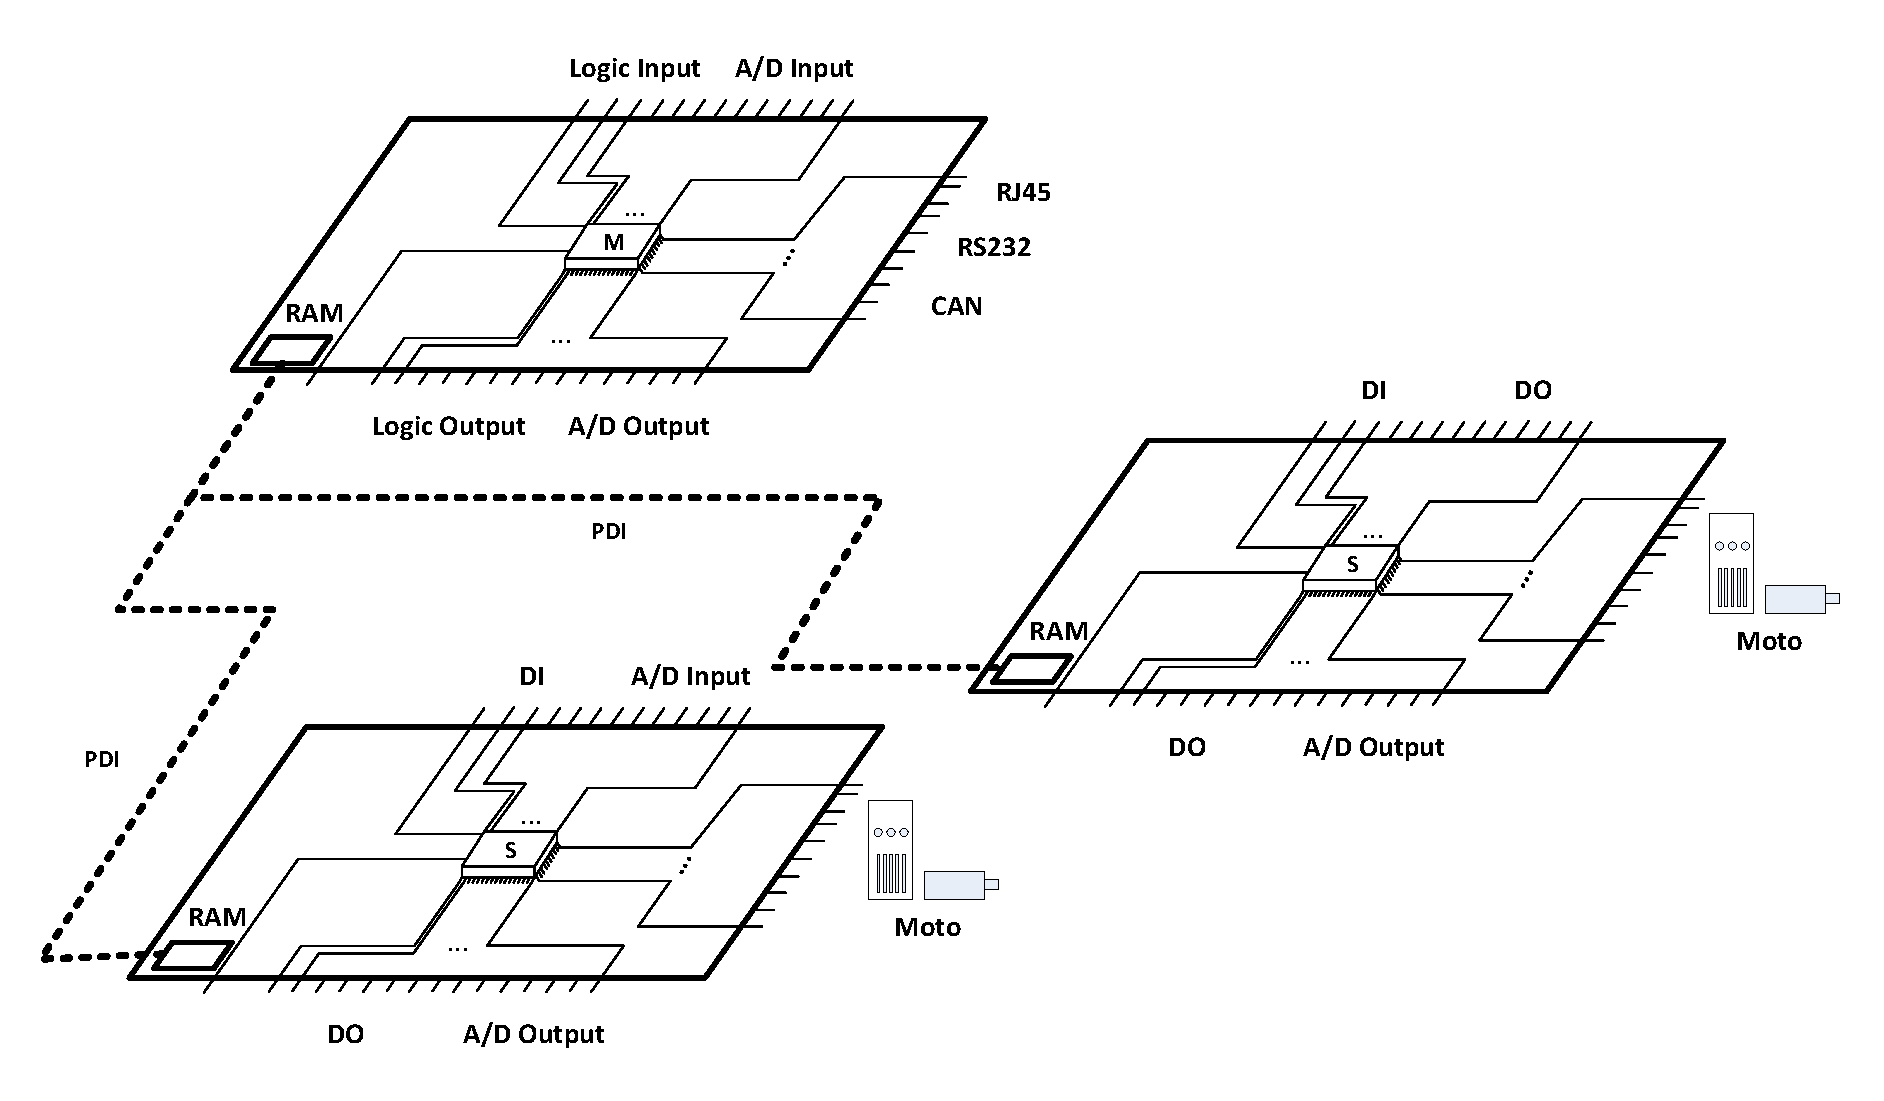
\includegraphics[width=3.5in]{fig/FIG2.pdf}
	\caption{ A type of hardware structure of multi-processor $ePLC$ which contains a master processor and two slave processors.}
	\label{fig:HardwareStructure}
\end{figure}
\subsection{Multi-language supported graphical component}
\label{component}
\begin{figure}
	\centering
	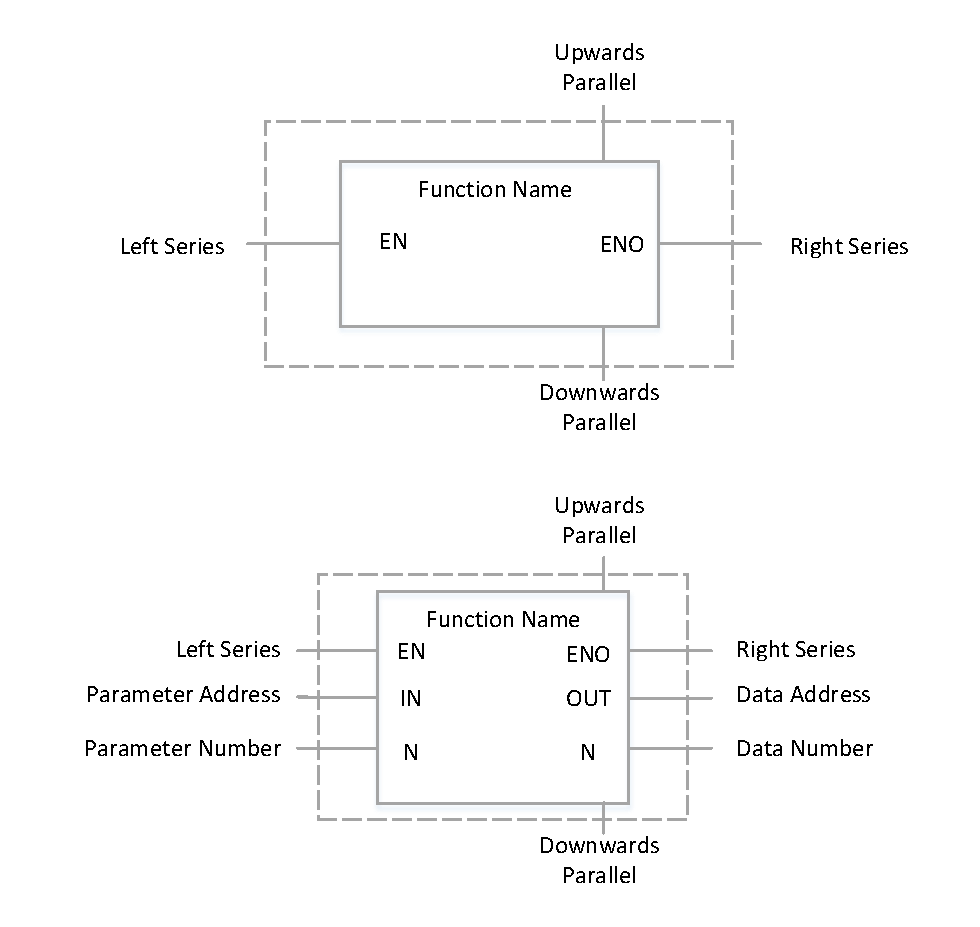
\includegraphics[width=3in]{fig/FIG6.pdf}
	\caption{ Two typical design: single component and component with input and output.}
	\label{fig:Component}
\end{figure}
In order to develop the logic program and algorithm program in the uniform platform. We package the algorithm into graphical component which is multi-language supported. The component is defined below.
\begin{equation}
LDC<Name,ID,PI,RI,PT,SF>
\end{equation} 
where:

\textbf{Name} is the name of component used to describe the function.

\textbf{ID} is the unique identifier of the component in the graphical program.

\textbf{PI} is a collection of service interfaces, including output data interfaces, right serial connection, downwards parallel connection and some auxiliary interfaces.

\textbf{RI} is a collection of requirement interfaces, including input data interfaces, left serial connection, downwards parallel connection and some auxiliary interfaces.

\textbf{PT} is an attribute collection of the component, including position, size, comment, etc.

\textbf{SF} is the function description explained by specific text, formula or frame template. The graphical basic component are divided into contact components, functional block components, coil components, cross line vertical components, change lines, comments, etc. The multi-language component specially includes the development language, the supported compiler and the executing processor.

Fig. \ref{fig:Component} illustrates two component design: single component and component with input and output. The single component has function name, left series, right series, upwards parallel and downwards parallel. In component with input and output, it contains function name, left series, right series, upwards parallel, downwards parallel, parameter address, parameter number, data address and data number.

As showed in Fig. \ref{fig:SoftwareStructure}, from the user's point of view, after inducing the multi-language component, the algorithm and logic program could be developed in a uniform $PLC$ platform. Multi-language components are supported by multiple languages such as IL instructions, ST language, C language, C++ language, etc. Algorithms contained in components are mainly motion control algorithms.
\begin{figure}
	\centering
	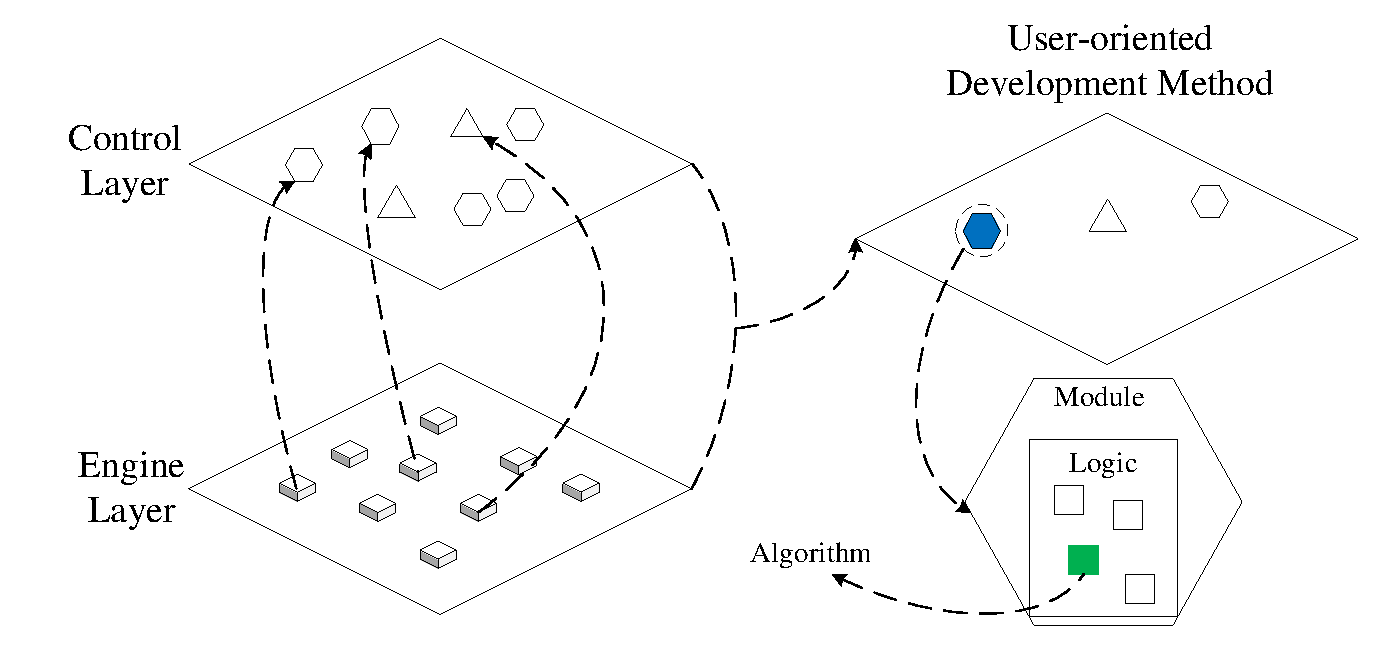
\includegraphics[width=3in]{fig/FIG3.pdf}
	\caption{ From the user's point of view, after inducing the multi-language component, the algorithm and logic program could be developed in a uniform $PLC$ platform.}
	\label{fig:SoftwareStructure}
\end{figure}


\begin{figure}
	\centering
	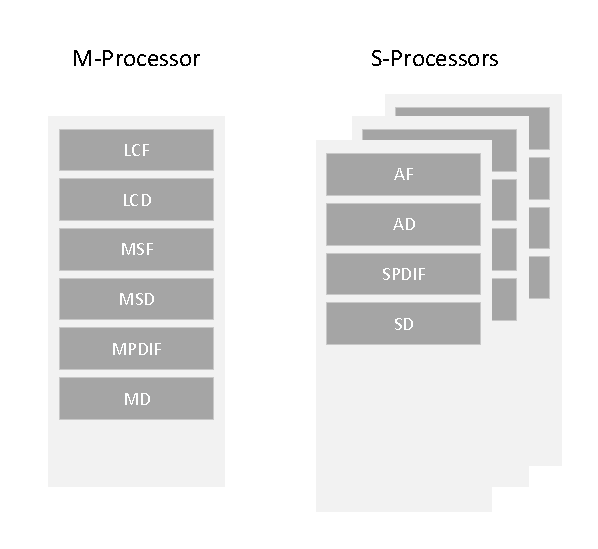
\includegraphics[width=3in]{fig/FIG4.pdf}
	\caption{ Memory allocation in master and slave processors.}
	\label{fig:Memory}
\end{figure}

\subsection{Memory Allocation}  

\textcolor{red}{The dedicated storage area of $PLC$ in memory is made up of bit data area ($M$ area) and byte data area ($D$ area). Meanwhile, we regard $M$ area and $D$ area as set $M$ of bit and set $D$ of byte. Furthermore, in this remaining paper, if $\exists$ set $T$, we describe its subscripted lowercase letter $t_i$ as an element of $T$ and the subscripted $i$ is used to distinguish the elements. Henceforth, two definitions are illustrated below.}

\textcolor{red}{\textbf{Definition 1} If $ T \subseteq M$, the value saved in $t_{i} \in \{0, 1\} $ and each element $t_i$ has four operators: $\mathcal{S}_0(t_i)$ denotes that $t_i$ is set to zero, $\mathcal{S}_1(t_i)$ denotes that $t_i$ is set to one, $\mathcal{J}_0(t_i)$ represents that the value of $t_i$ is judged as $0$, $\mathcal{J}_1(t_i)$ represents that the value of $t_i$ is judged as $1$. Then we define the set $T$ has $\mathcal{B}$ attribute.}

\textcolor{red}{\textbf{Definition 2} If $ T \subseteq D$ and $\forall t_{i} \in T$ has 4 bytes. We define the set $T$ has $\mathcal{D}$ attribute.}


Fig. \ref{fig:Memory} shows the memory allocation of master and slave processors. All slave processors have the same storage structure.

\textbf{\emph{LCF}} (Logic Control Flag Area): the flag are used to start the modules. It has $\mathcal{B}$ attribute.

\textbf{\emph{LCD}} (Logic Control Data Area): these data will be used to delivery to algorithm. It has $\mathcal{D}$ attribute.

\textbf{\emph{AF}} (Algorithm Flag Area): it includes algorithm flag of execution ($AFE$) and algorithm flag of state ($AFS$). Both of them have $\mathcal{B}$ attribute.

\textbf{\emph{AD}} (Algorithm Data Area): these data help specified algorithm executing. It has $\mathcal{D}$ attribute.

\textbf{\emph{MF}} (Message Flag Area): it includes defined message flag ($DMF$) and user customized message flag ($UMF$). $DMF$ is the necessary message for system execution, e.g. start module flag, alarm flag, etc. $UMF$ could be defined by users. Both of them have $\mathcal{B}$ attribute.

\textbf{\emph{MD}} (Message Data Area): it is used to transfer message information which includes system message data area ($DMD$) and usr message data area ($UMD$). It is defined in $D$ area.

\textbf{\emph{MPDIF}} (Master Processor Data Interaction Flag Area): it contains begin data transfer flag from master to slave ($MSB$), transfer state of master from master to slave ($MSF$), acknowledge flag of master from master to slave ($MSA$) and transfer state of master from slave to master ($MSS$). All of them have $\mathcal{B}$ attribute.

\textbf{\emph{MSD}} (Master Processor Data Interaction Data Area): an area stores the data delivered from slave processors and it has $\mathcal{D}$ attribute.

\textbf{\emph{SPDIF}} (Slave Processor Data Interaction Flag Area): this area includes the begin data transfer flag from slave to master ($SMB$), transfer state of slave from slave to master ($SMF$), acknowledge flag of slave from slave to master ($SMA$) and transfer state of slave from master to slave ($SMS$). All of them have $\mathcal{B}$ attribute.

\textbf{\emph{SMD}} (Slave Processor Data Interaction Data Area): an area stores the data delivered from master processor and it has $\mathcal{D}$ attribute.

\subsection{User-oriented Thread Design}
From the user's point of view, in most cases, the logic control program ($LCP$) and algorithm program ($AP$) could be developed independently \cite{WuA}, hence we have logic thread and algorithm thread. On the other hand, in order to satisfying ever-growing performance requirement of users, we proposed the customized multi-processor $ePLC$. Correspondingly an individual motion thread is designed into every slave processor. The user-oriented thread structure can be seen in Fig \ref{fig:Threads}. Every processor is a four level preemptive scheduling thread structure. \textbf{Emergent Thread}, \textbf{Communication Thread}, \textbf{Diagnose Thread} and \textbf{APC Thread} see in \cite{WuA}. Two special threads are explained below.

\textbf{Control Thread}: it is running in master processor and has functions including dealing with DI$\backslash$O, executing logic program, exchanging data with slave processors, etc.

\textbf{Algorithm Thread}: it is running in slave processor and contains functions including interacting data with master, executing algorithm program, controlling actuators, etc.

\subsection{Modular Design}  
\textcolor{red}{In applications, modular design will reduce the complexity of program \cite{Vyatkin2013Software}.} Therefore, we provide a system level frame for modular design. In Fig. \ref{fig:SoftwareStructure}, we can have a look on the modular design. The program is composed by a lot of modules and a module consists of logic program and several related algorithms. Modules will work under the reasonable memory allocation, data interaction mechanism and running multithreading. Hence, we could define a program of $ePLC$ as follows.

\begin{equation}
	\left\{
	\begin{array}{l}
	PS = \{MS, MA , LPM, TD\}\\
	ms_i \in MS = \{lcp_i, \bigcup_{j=g}^h ap_j\}\\
	lcp_i \in LCP = \{ip_i, lcf_i, lcd_i, lpb_i\}\\
	ap_j \in AP = \{afe_j, afs_j, ad_j, ab_j\}
	\end{array}
	\right.
	\end{equation}

The programming structure ($PS$) consists of modules ($MS$), memory allocation ($MA$), $LPM$ data interaction and threads ($TD$). Each $ms_i$ has two parts: logic control program $lcp_i$ and several algorithm programs ($ap_g, ap_{g+1},..., ap_{j},..., ap_{h}$). Each $lcp_i$ includes initial program ($ip_i$), logic control flag ($lcf_i$), logic control data ($lcd_i$) and logic program body ($lpb_i$). Each $ap_{j}$ contains $afe_{j}$, $afs_{j}$, $ad_{j}$ and algorithm body ($ab_{j}$).

\begin{figure}
	\centering
	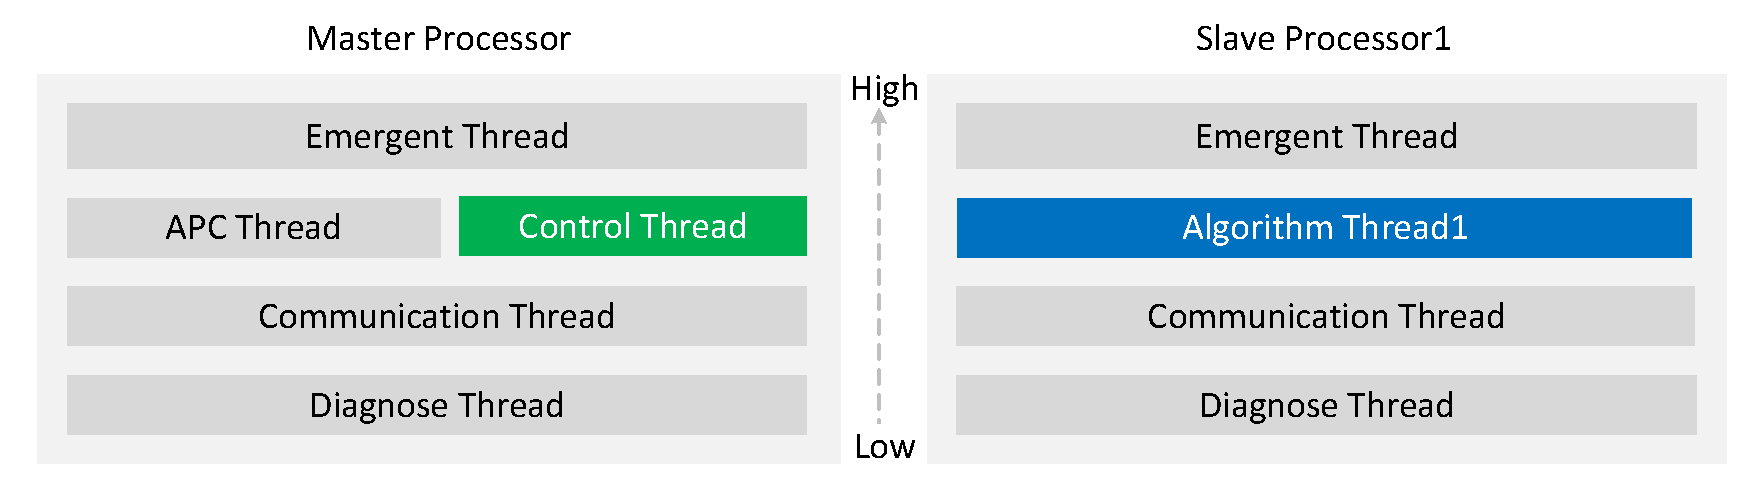
\includegraphics[width=3in]{fig/FIG5.pdf}
	\caption{ User-oriented thread design in master and slave processors.}
	\label{fig:Threads}
\end{figure}
 \section{System Implementation}
 \label{Process}
 \subsection{Compilation of the graphic program}
The compilation contains two parts: compiling graphic language into instruction list and compiling the multi-language components.
 	
  In the first part, since we see the multi-language components as an common component, the compilation of graphic language embedded multi-language components is almost the same with the process of \cite{Yan2010Compiling} in which you can find the detailed explanation. As an example shown in Fig. \ref{fig:Compile}, we adopt three steps to implement it:
 	
 \textbf{Step 1}: convert topology structure to directed graph according to ladder diagram syntax library and analyze the errors of the topology.
 	
 \textbf{Step 2}: generate a binary decomposition tree according to series and parallel rules.
 	
 \textbf{Step 3}: generate IL instructions according to the IL grammar library. For multi-language components, it is described as a program entry.
 
 \begin{figure}
 	\centering
 	\includegraphics[width=3in]{fig/Compile.pdf}
 	\caption{Three steps of compilation of graphic program which contains multi-language component: convert topology structure to directed graph, generating a binary decomposition tree and generating IL instructions.}
 	\label{fig:Compile}
 \end{figure}
 
 In the second part, the multi-language components will be compiled. For the convenience of users, they can still use the same grammar to program the $ePLC$ dedicated storage area inside the multi-language component, such as $M2000=1$ which represents to give $1$ to the bit area $M2000$, whereas it is illegal in other languages. Hence, we should compile the component to the identifiable code which contains two steps.
 	
\textbf{Step 1}: address mapping. Every type of processor has its own address mapping rules ($AMR$).
 \begin{eqnarray}
  APR = \{CID, MAS, DAS, \mathcal{A}_m, \mathcal{A}_d\}
 \end{eqnarray}
 Where $CID$ is the compiler identity, $MAS$ and $DAS$ are the start address of $M$ and $D$ area, respectively. $\mathcal{A}_m$ and $\mathcal{A}_d$ are the rules to map the $M$ and $D$ to the address of processor, respectively, \textcolor{red}{see Algorithm \ref{alg1} and Algorithm \ref{alg2}. Algorithm \ref{alg1} translates the four operators of each element $m_i$, which are $\mathcal{S}_0(m_i)$, $\mathcal{S}_1(m_i)$, $\mathcal{J}_0(m_i)$, $\mathcal{J}_1(m_i)$, to recognizable form of $CID$ compiler. In addition, in $PLC$ platform, we adopt the octal system so it is necessary to translate the octal number to decimal number. Algorithm \ref{alg1} and Algorithm \ref{alg2} both contain this process.
 }
 
\textbf{Step 2}: call the corresponding compiler to compile the component.


\begin{algorithm}
	\label{alg1}
	\caption{$\mathcal{A}_m$}%算法名字
	%\LinesNumbered %要求显示行号
	\KwIn{string oStr of $m_i$ contained its operator}%输入参数
	\KwOut{converted string cStr}%输出
	Get the number $i$ from oStr\; 
	Get operator $opt$ from oStr\;
	remainder r = $i\%10$\;
	Octal oI =  $i/10$\;
	Convert oI to decimal dI\; 
	\For{opt}{
		\If{opt==$\mathcal{S}_0$}{
			cStr = "CassMen[$MAS$+dI] $\gg$ r == 0"\;
		}
		\If{opt==$\mathcal{S}_1$}{
        	cStr = "CassMen[$MAS$+dI] $\gg$ r == 1"\;
       }		
		\If{opt==$\mathcal{J}_0$}{
	       cStr = "CassMen[$MAS$+dI] $\mid \sim$(1 $\ll$ r)"\;
       }
       \If{opt==$\mathcal{J}_1$}{
           cStr = "CassMen[$MAS$+dI] \& (1 $\ll$ r)"\;
       }	  	    
	}
\end{algorithm}
\begin{algorithm}
	\label{alg2}
	\caption{$\mathcal{A}_d$}%算法名字
	%\LinesNumbered %要求显示行号
	\KwIn{string oStr of $d_i$}%输入参数
	\KwOut{converted string cStr}%输出
	Get the number $i$ from oStr\; 
	Convert $i$ to decimal dI\; 
	cStr = "CassMen[$DAS$+dI]"\;
\end{algorithm}


 
 \subsection{LPM data interaction}
 As shown in Fig. \ref{fig:Interaction}, we define the $LPM$ data interaction with three parts: $\mathcal{L}$ (layer data interaction), $\mathcal{P}$ (processor data interaction) and $\mathcal{M}$ (module data interaction). $\mathcal{L}$ seen in \cite{WuA} is the process to exchange the data between application customized layer and control layer.

$\mathcal{P}$ is used to interact data between master processor and slave processors, hence it has the process of transferring data from master to slave ($\mathcal{P}_{mts}$) and the process of transferring data from slave to master ($\mathcal{P}_{stm}$) which are defined below:
 \begin{equation}
 \left\{
 \begin{array}{l}
 \mathcal{P}_{mts} = \mathcal{U} (msb_i,msf_i,sma_i,sms_i,smd_i)\\
 \mathcal{P}_{stm} = \mathcal{U} (smb_i,smf_i,msa_i,mss_i,msd_i)
 \end{array}
 \right.
 \end{equation}
Where $\mathcal{U}$ is the function to implement the process of data interaction between master and slave processors. $\mathcal{P}_{mts}$ and $\mathcal{P}_{mts}$ use the same function $\mathcal{U}$.

 The process flow of $\mathcal{P}_{mts}$ is denoted below:
 $\mathcal{S}_1(msb_i)\to\mathcal{S}_1(msf_i)\to send(smd_i)\to\mathcal{S}_0(msb_i)\to\mathcal{S}_1(sms_i)\to check(smd_i)\to\mathcal{S}_1(sma_i)\to\mathcal{S}_0(sms_i)\to\mathcal{S}_0(sma_i)\to\mathcal{S}_0(msf_i)$.
 
\textcolor{red}{Here $send(msd_i)$ denotes sending data to $msd_i$ in slave processor. $check(msd_i)$ denotes to check data of $msd_i$. $\to$ denotes the transition to the next step, e.g. $\mathcal{S}_1(msb_i)\to\mathcal{S}_1(msf_i)$ denotes $msb_i$ is set one and then $msf_i$ is set one.}
 
$\mathcal{M}$ is used to interact data among modules. It includes two type messages: system defined message interaction $\mathcal{M}_{d}$ and user message interaction $\mathcal{M}_{u}$. The process is defined below:
 \begin{equation}
\left\{
\begin{array}{l}
\mathcal{M}_{d} = \mathcal{V} (dmf_i,dmd_i,\mathcal{E})\\
\mathcal{M}_{u} = \mathcal{V} (umf_i,umd_i\,\mathcal{E})
\end{array}
\right.
\end{equation}
Where $\mathcal{V}$ is the function to broadcast message and transfer data. $\mathcal{E}$ is the collection of all execution functions after getting related message, $\mathcal{M}_{s}$ and $\mathcal{M}_{u}$ have the same function $\mathcal{V}$.

One module receives a system defined message shown below:
$\mathcal{J}_1(smf_i)\to GetMessage_{j}(dmf_i)\to GetData(dmd_i)\to\mathcal{E}_j$.

 Here $GetMessage_{j}(dmf_i)$ represents the $i$th module getting a message $dmf_i$ and $GetData(dmd_i)$ represents the $i$th module getting the message information.

 \begin{figure}
	\centering
	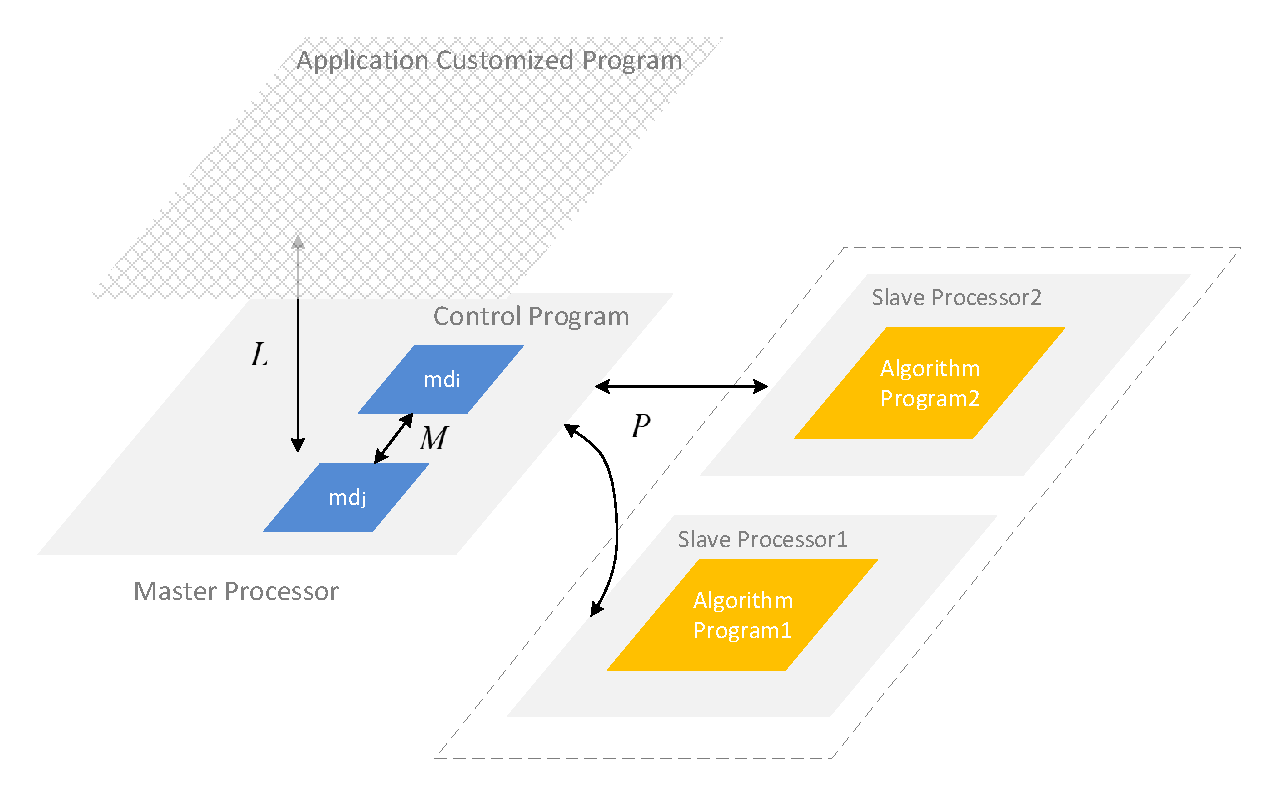
\includegraphics[width=3in]{fig/Interaction.pdf}
	\caption{ $LPM$ data interaction is defined with three parts: $\mathcal{L}$ (layer data interaction), $\mathcal{P}$ (processor data interaction) and $\mathcal{M}$ (module data interaction).}
	\label{fig:Interaction}
\end{figure}

 \subsection{Execution of Threads}
 Commonly, threads in master processor and in slave processors execute separately according to their priority and the interaction between control thread and algorithm threads occurs when using $\mathcal{P}_{mts}$ and $\mathcal{P}_{mts}$. Basic execution units of control thread are shown as follows:
 
 \textbf{$C_{1}$}: start a module.
 
 \textbf{$C_{2}$}: transfer data to slave processor by $\mathcal{P}_{mts}$.
 
 \textbf{$C_{3}$}: deal with the feedback data.
 
 \textbf{$C_{4}$}: broadcast a message.
 
  \textbf{$C_{5}$}: handle the message.
  
 Motion thread contains the following basic execution units:
 
 \textbf{$M_{1}$}: start the algorithm.
 
 \textbf{$M_{2}$}: execute the algorithm.
 
 \textbf{$M_{3}$}: feedback the data to master processor by $\mathcal{P}_{stm}$.
 
 \textbf{$M_{4}$}: end algorithm.
  
  Two cases shown in Fig. \ref{fig:threadFlow} are explained below:
  
  \textbf{Case one}: the execution of control thread and two algorithm threads among three processors. The control thread ($CT$) traverses $LCF$, finds $ms_i$ to be executed , runs $lcp_i$, finds $ap_j$, executes $C_1$ unit, executes $C_2$ unit and then transfers data from $LCD$ to $SMD$ of processor 1. Algorithm thread ($AT$) 1 executes $M_1$ unit, executes $M_2$ after transferring data from $SMD$ to $AD$, runs $M_3$ unit, feedbacks data to $CT$. When the $ap_j$ finishes, $AT$ 1 executes $M_4$ and informs $CT$ the end of $ap_j$. $CT$ executes $C_3$ to end the process and then finds $ap_{j+1}$, executes $C_1$ and $C_2$, transfers the data from $LCD$ to $SMD$ of processor 2, $AT$ 2 executes $M_1$ unit, executes $M_2$ after transferring data from $SMD$ to $AD$. When the $ap_{j+1}$ finishes, $AT$ 2 executes $M_4$ unit and informs $CT$ the end of $ap_{j+1}$. $CT$ executes $C_3$ to finish the process.
  
  \textbf{Case two}: the execution of control thread and two algorithm threads among three processors together with message mechanism. The $CT$ traverses $LCF$, finds $ms_i$ to be executed , runs $lcp_i$, finds $ap_j$, executes $C_1$ unit, executes $C_2$ unit and then transfers data from $LCD$ to $SMD$ of processor 1. $AT$ 1 executes $M_1$ unit, executes $M_2$ after transferring data from $SMD$ to $AD$. During the execution of $ms_i$, $CT$ executes $C_4$ to broadcast the message $dmf_x$ to inform $ms_{k}$ to run. After executing of $C_5$, $ms_{k}$ gets data and start, then $CT$ finds $ap_{j+1}$ in $ms_{k}$, executes $C_1$ and $C_2$, transfers the data from $LCD$ to $SMD$ of processor 2, $AT$ 2 executes $M_1$ unit, executes $M_2$ after transferring data from $SMD$ to $AD$. During the execution of $ap_{j+1}$, $AT$ 1 executes $M_4$ and informs $CT$ to execute $C_3$. After that, $ap_{j+1}$ finishes, then $CT$ executes $C_3$ to finish the process.
  

  
  \begin{figure}
  	\centering
  	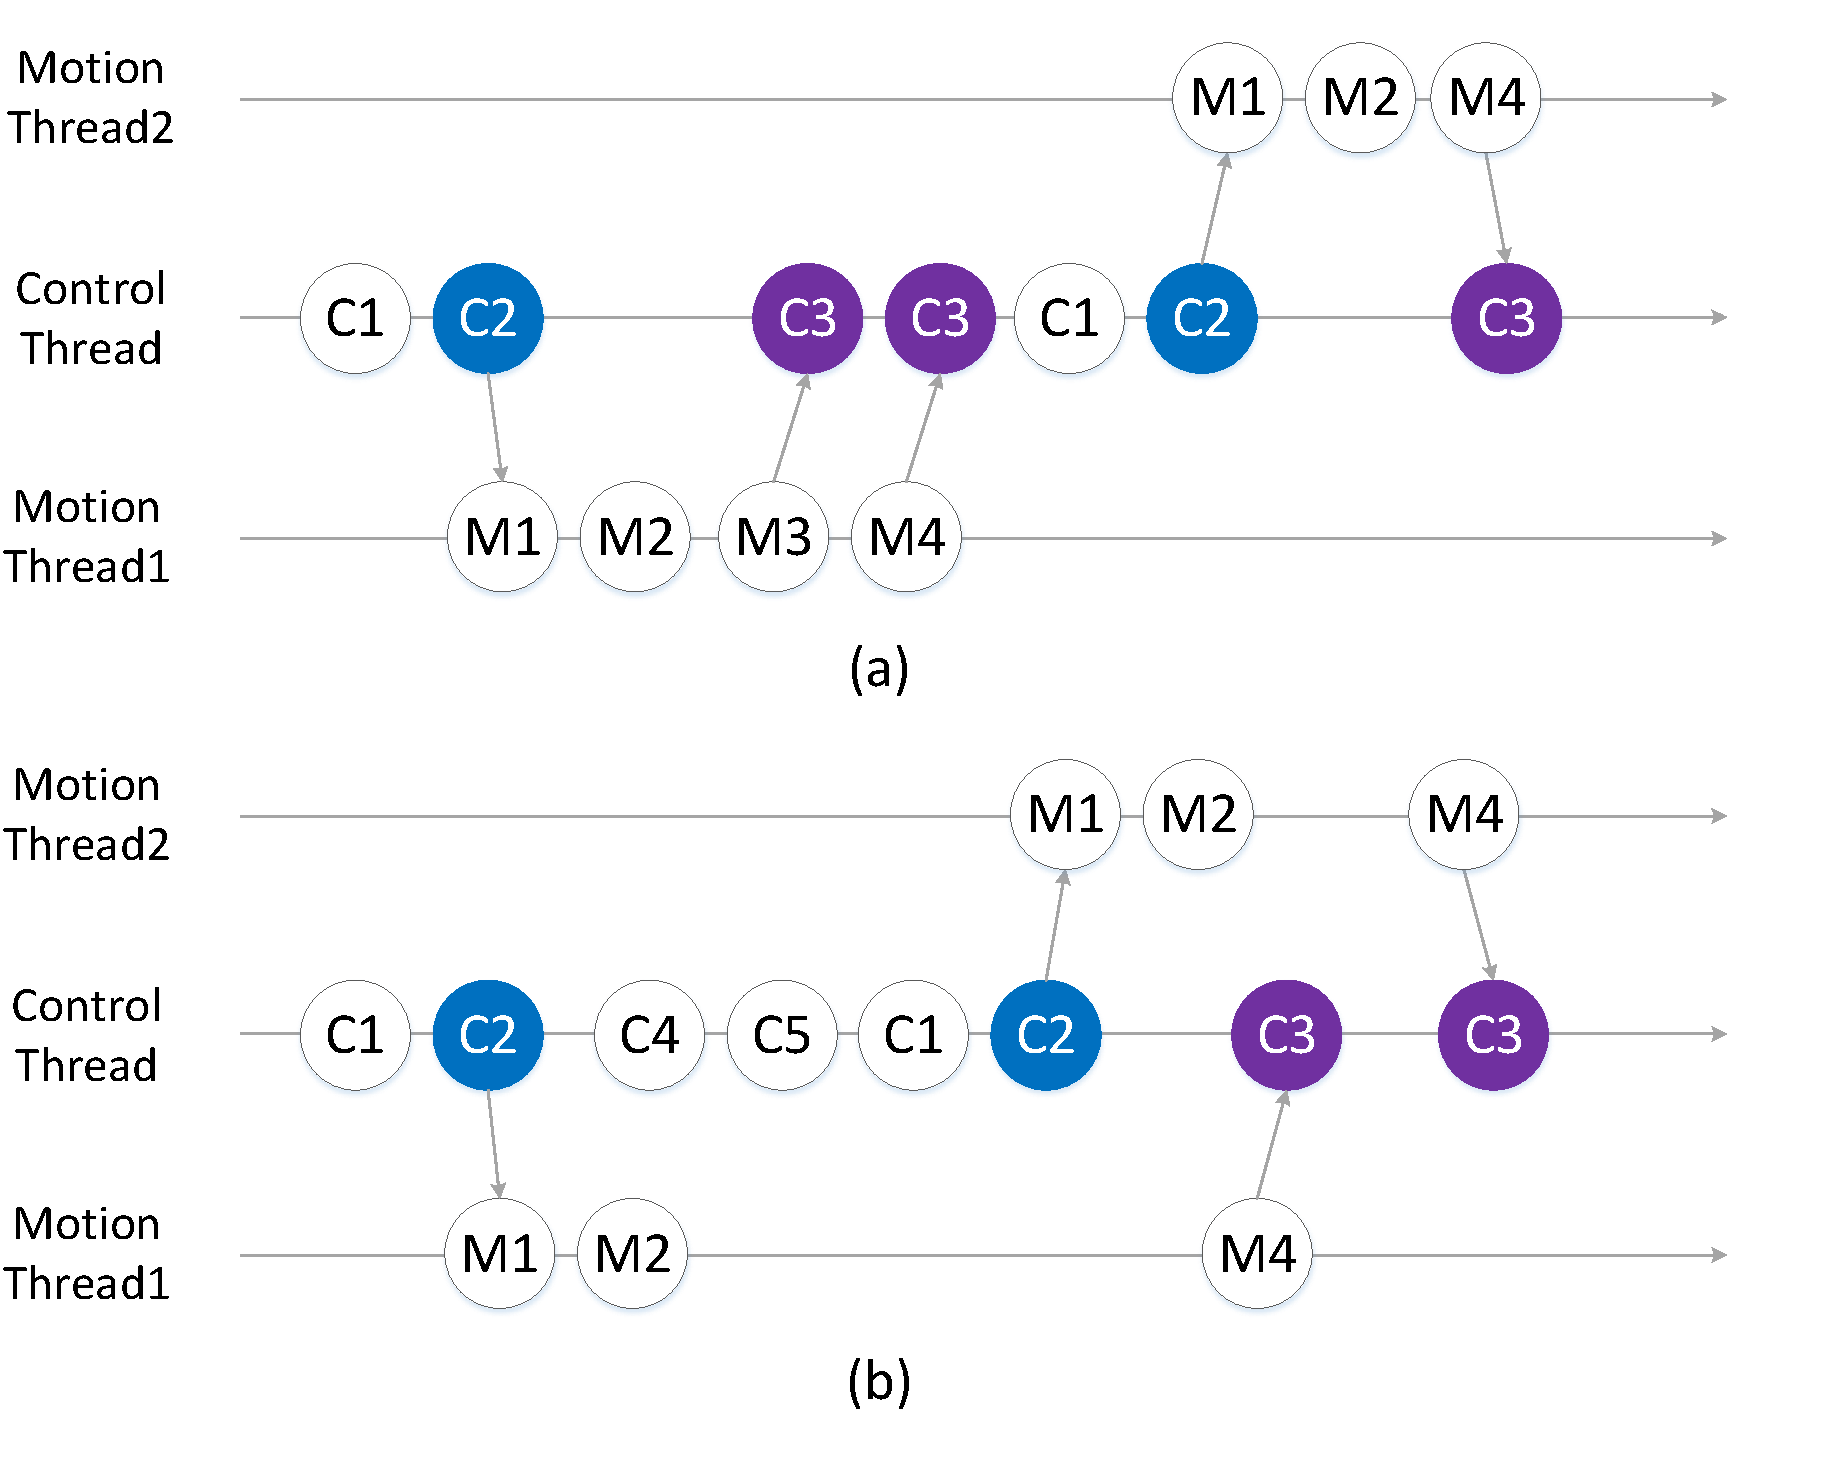
\includegraphics[width=3in]{fig/threadFlow.pdf}
  	\caption{ Execution of control thread and two algorithm threads among three processors with and without message.}
  	\label{fig:threadFlow}
  \end{figure}
 \subsection{Finite State Machines}
 \textcolor{red}{ The finite state machines adopt the 5-tuple which is similar with \cite{Hierons2016Parallel}:
 \begin{equation}
 \mathcal{F} = (Q, X, Y, \delta, \lambda)
 \end{equation}
 Where $Q = \{q_0, q_1,..., q_i\}$ is the collection of states, $q_0 \in Q$ is the initial state. $X$ is the finite set of inputs. $Y$ is the finite set of outputs. $\delta$ is the state transition function $\delta: Q\times X \rightarrow Q$. $\lambda$ is the output function $\lambda: Q\times X\rightarrow Y$. If $F$ is in state $q$ and $x$ is occurred, then the $F$ transits to state $q' = \delta(q, x)$ and outputs $y = \lambda(q, x)$. This transition could be denoted $\tau = (s,x/o,s')$.}
 
 \textcolor{red}{Hence, we have the following finite state machines of master processor:
  \begin{equation}
  \label{FMaster}
 \left\{
 \begin{array}{l}
 \mathcal{F}_{m} = \{Q_m, X_m, Y_m,\delta_m, \lambda_m\}\\
 Q_m = \{mstop, mrun, mbm, pdi\}\\
 X_m = \{x_{m1}, x_{m2}, x_{m3}, x_{m4}, x_{m5}, x_{m6}, x_{m7}\}\\
 Y_m = \{y_{m1}, y_{m2}, y_{m3}\}
 \end{array}
 \right.
 \end{equation}
 Where, $mstop$ is the stop state and the initial state of master processor, $mrun$ is the run state, $mbm$ is the broadcast state and $pdi$ is the data interaction state. The inputs are defined below:
 \begin{align}
 \notag x_{m1}&\Leftrightarrow \exists lcf_i: \mathcal{J}_1(lcf_i)\\
\notag x_{m2}&\Leftrightarrow  \forall lcf_i: \mathcal{J}_0(lcf_i)\\
\notag x_{m3}&\Leftrightarrow \exists mf_i: \mathcal{J}_1(mf_i)\\
\notag x_{m4}&\Leftrightarrow \forall mf_i: \mathcal{J}_0(mf_i)\\
\notag x_{m5}&\Leftrightarrow \exists msf_i, mss_j: \mathcal{J}_1(msf_i) \lor \mathcal{J}_1(mss_j)\\
\notag x_{m6}&\Leftrightarrow \forall msf_i, mss_j, mf_k: \mathcal{J}_0(msf_i) \land \mathcal{J}_0(mss_j) \land \mathcal{J}_0(mf_k)\\
\notag x_{m7}&\Leftrightarrow \forall msf_i, mss_j, \exists mf_k: \mathcal{J}_0(msf_i) \land \mathcal{J}_0(mss_j) \land \mathcal{J}_1(mf_k)\\
\notag y_{m1}&\Leftrightarrow C_1\\
\notag y_{m2}&\Leftrightarrow C_4\\
\notag y_{m3}&\Leftrightarrow C_2\quad or\quad C_3
 \end{align}}
\textcolor{red}{Here, e.g. $x_{m1}\Leftrightarrow \exists lcf_i: \mathcal{J}_1(lcf_i)$ denotes that $x_{m1}$ is an input of the $X_m$ and this input equivalent to the existence of an logic control flag, $lcf_i$ whose value is 1.}

\textcolor{red}{Then we can get the state transitions of master processor:
  \begin{equation}
 \left\{
 \begin{array}{l}
 \tau_m1 = (mstop, x_{m1}/y_{m1}, mrun)\\
 \tau_m2 = (mrun, x_{m2}, mstop)\\
 \tau_m3 = (mrun, x_{m3}/y_{m2}, mbm)\\
 \tau_m4 = (mbm, x_{m4}, mrun)\\
 \tau_m5 = (mrun, x_{m5}/y_{m3}, pdi)\\
 \tau_m6 = (pdi, x_{m6}, mrun)\\
 \tau_m7 = (mbm, x_{m5}/y_{m3}, pdi)\\
 \tau_m8 = (pdi, x_{m7}, mbm)\\
 \end{array}
 \right.
 \end{equation}}
 
 
 \textcolor{red}{The finite state machines of every slave processor are illustrated below:
 \begin{equation}
 \label{FSlave}
 \left\{
 \begin{array}{l}
 \mathcal{F}_{s} = \{Q_s, X_s, Y_s, \delta_s, \lambda_s\}\\
 Q_s = \{sstop, sready, srun, pdi\}\\
 X_s = \{x_{s1}, x_{s2}, x_{s3}, x_{s4}, x_{s5}\}\\
 Y_s = \{y_{s1}, y_{s2}, y_{s3}\}\\
 \end{array}
 \right.
 \end{equation}
 where $sstop$ is the stop state and the initial state, $srun$ is the run state, $sready$ is the ready state and $pdi$ is the data interaction state. The events are defined below:
\begin{align}
\notag x_{s1}&\Leftrightarrow \exists sms_i: \mathcal{J}_1(sms_i)\\
\notag x_{s2}&\Leftrightarrow \exists afe_i: \mathcal{J}_1(afe_i)\\
\notag x_{s3}&\Leftrightarrow \exists afs_i: \mathcal{J}_1(afs_i)\\
\notag x_{s4}&\Leftrightarrow \forall afs_i: \mathcal{J}_0(afs_i)\\
\notag x_{s5}&\Leftrightarrow \exists smb_i, sms_j: \mathcal{J}_1(smb_i) \lor \mathcal{J}_1(sms_j)\\
\notag y_{s1}&\Leftrightarrow M_1\\
\notag y_{s2}&\Leftrightarrow M_2\\
\notag y_{s3}&\Leftrightarrow M_3
\end{align}}

 
 \textcolor{red}{Then we can get the state transitions of slave processor:
 \begin{equation}
 \left\{
 \begin{array}{l}
 \tau_{s1} = (sstop, x_{s1}/y_{s1}, pdi)\\
 \tau_{s2} = (pdi, x_{s2}, sready)\\
 \tau_{s3} = (sready, x_{s3}/y_{s2}, srun)\\
 \tau_{s4} = (srun, x_{s4}, sstop)\\
 \tau_{s5} = (srun, x_{s5}/y_{s3}, pdi)
 \end{array}
 \right.
 \end{equation}}

\textcolor{red}{Fig. \ref{fig:state} illustrates the whole finite state machines of $ePLC$ which contains master processor $M$, slave processor $S_1$ and slave processor $S_i$. This is the figure form of Eq. \ref{FMaster} and Eq. \ref{FSlave}. }
 \begin{figure}
	\centering
	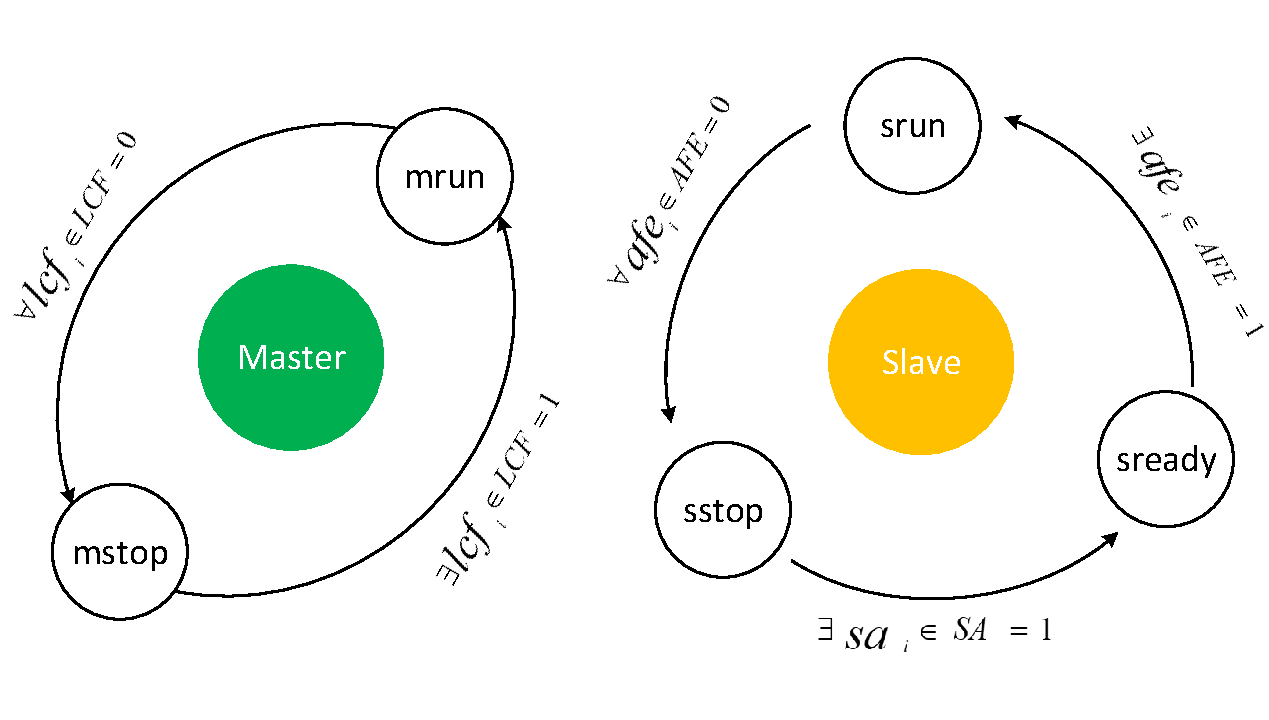
\includegraphics[width=3in]{fig/state.pdf}
	\caption{ Finite state machines of $ePlC$ which contains master processor $M$, slave processor $S_1$ and slave processor $S_i$.}
	\label{fig:state}
\end{figure}
\section{Experiment}
\label{Experiment}

\begin{figure}
	\centering
	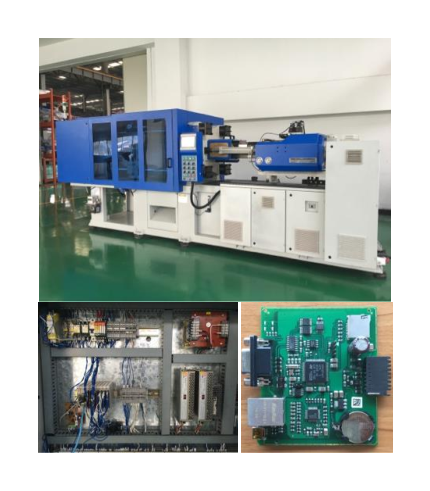
\includegraphics[width=3in]{fig/FIG10.pdf}
	\caption{200 ton injection molding machine and its control distributed system.}
	\label{fig:IMM}
\end{figure}

\subsection{Distributed Control System}
As show in Fig. \ref{fig:IMM}, we verify the proposal development method on a 200 ton $IMM$. The TI F28M35 chip is chosen as the main chip of $ePLC$. It has two cores: a TI C28x and an ARM Cortex M3. Considering the DSP is more suitable for motion control, Cortex M3 is chosen as master processor and C28x is chosen as slave processor. The $ePLC$ has a RJ45, a RS232 and a CAN. RJ45 is used to download program, RS232 is for connecting with HMI and CAN is designed to extend the DI$\backslash$O and AI$\backslash$O. The $HMI$ could be customized by users.

\subsection{Software Structure}
Fig. \ref{fig:ld} shows uniform development platform developed by ourselves. In the dotted line box of Fig. \ref{fig:ld} (a), it is the C language component and Fig. \ref{fig:ld} (b) is its partial code. This component represents to output a small velocity and pressure in setup mode.

After the design of every used components, we design the modules according to Table \ref{table:IMMSystem}. Additionally, a special module is designed to control the execution flow of all modules with the $DMF$ and $DMD$.

\begin{figure}
	\centering
	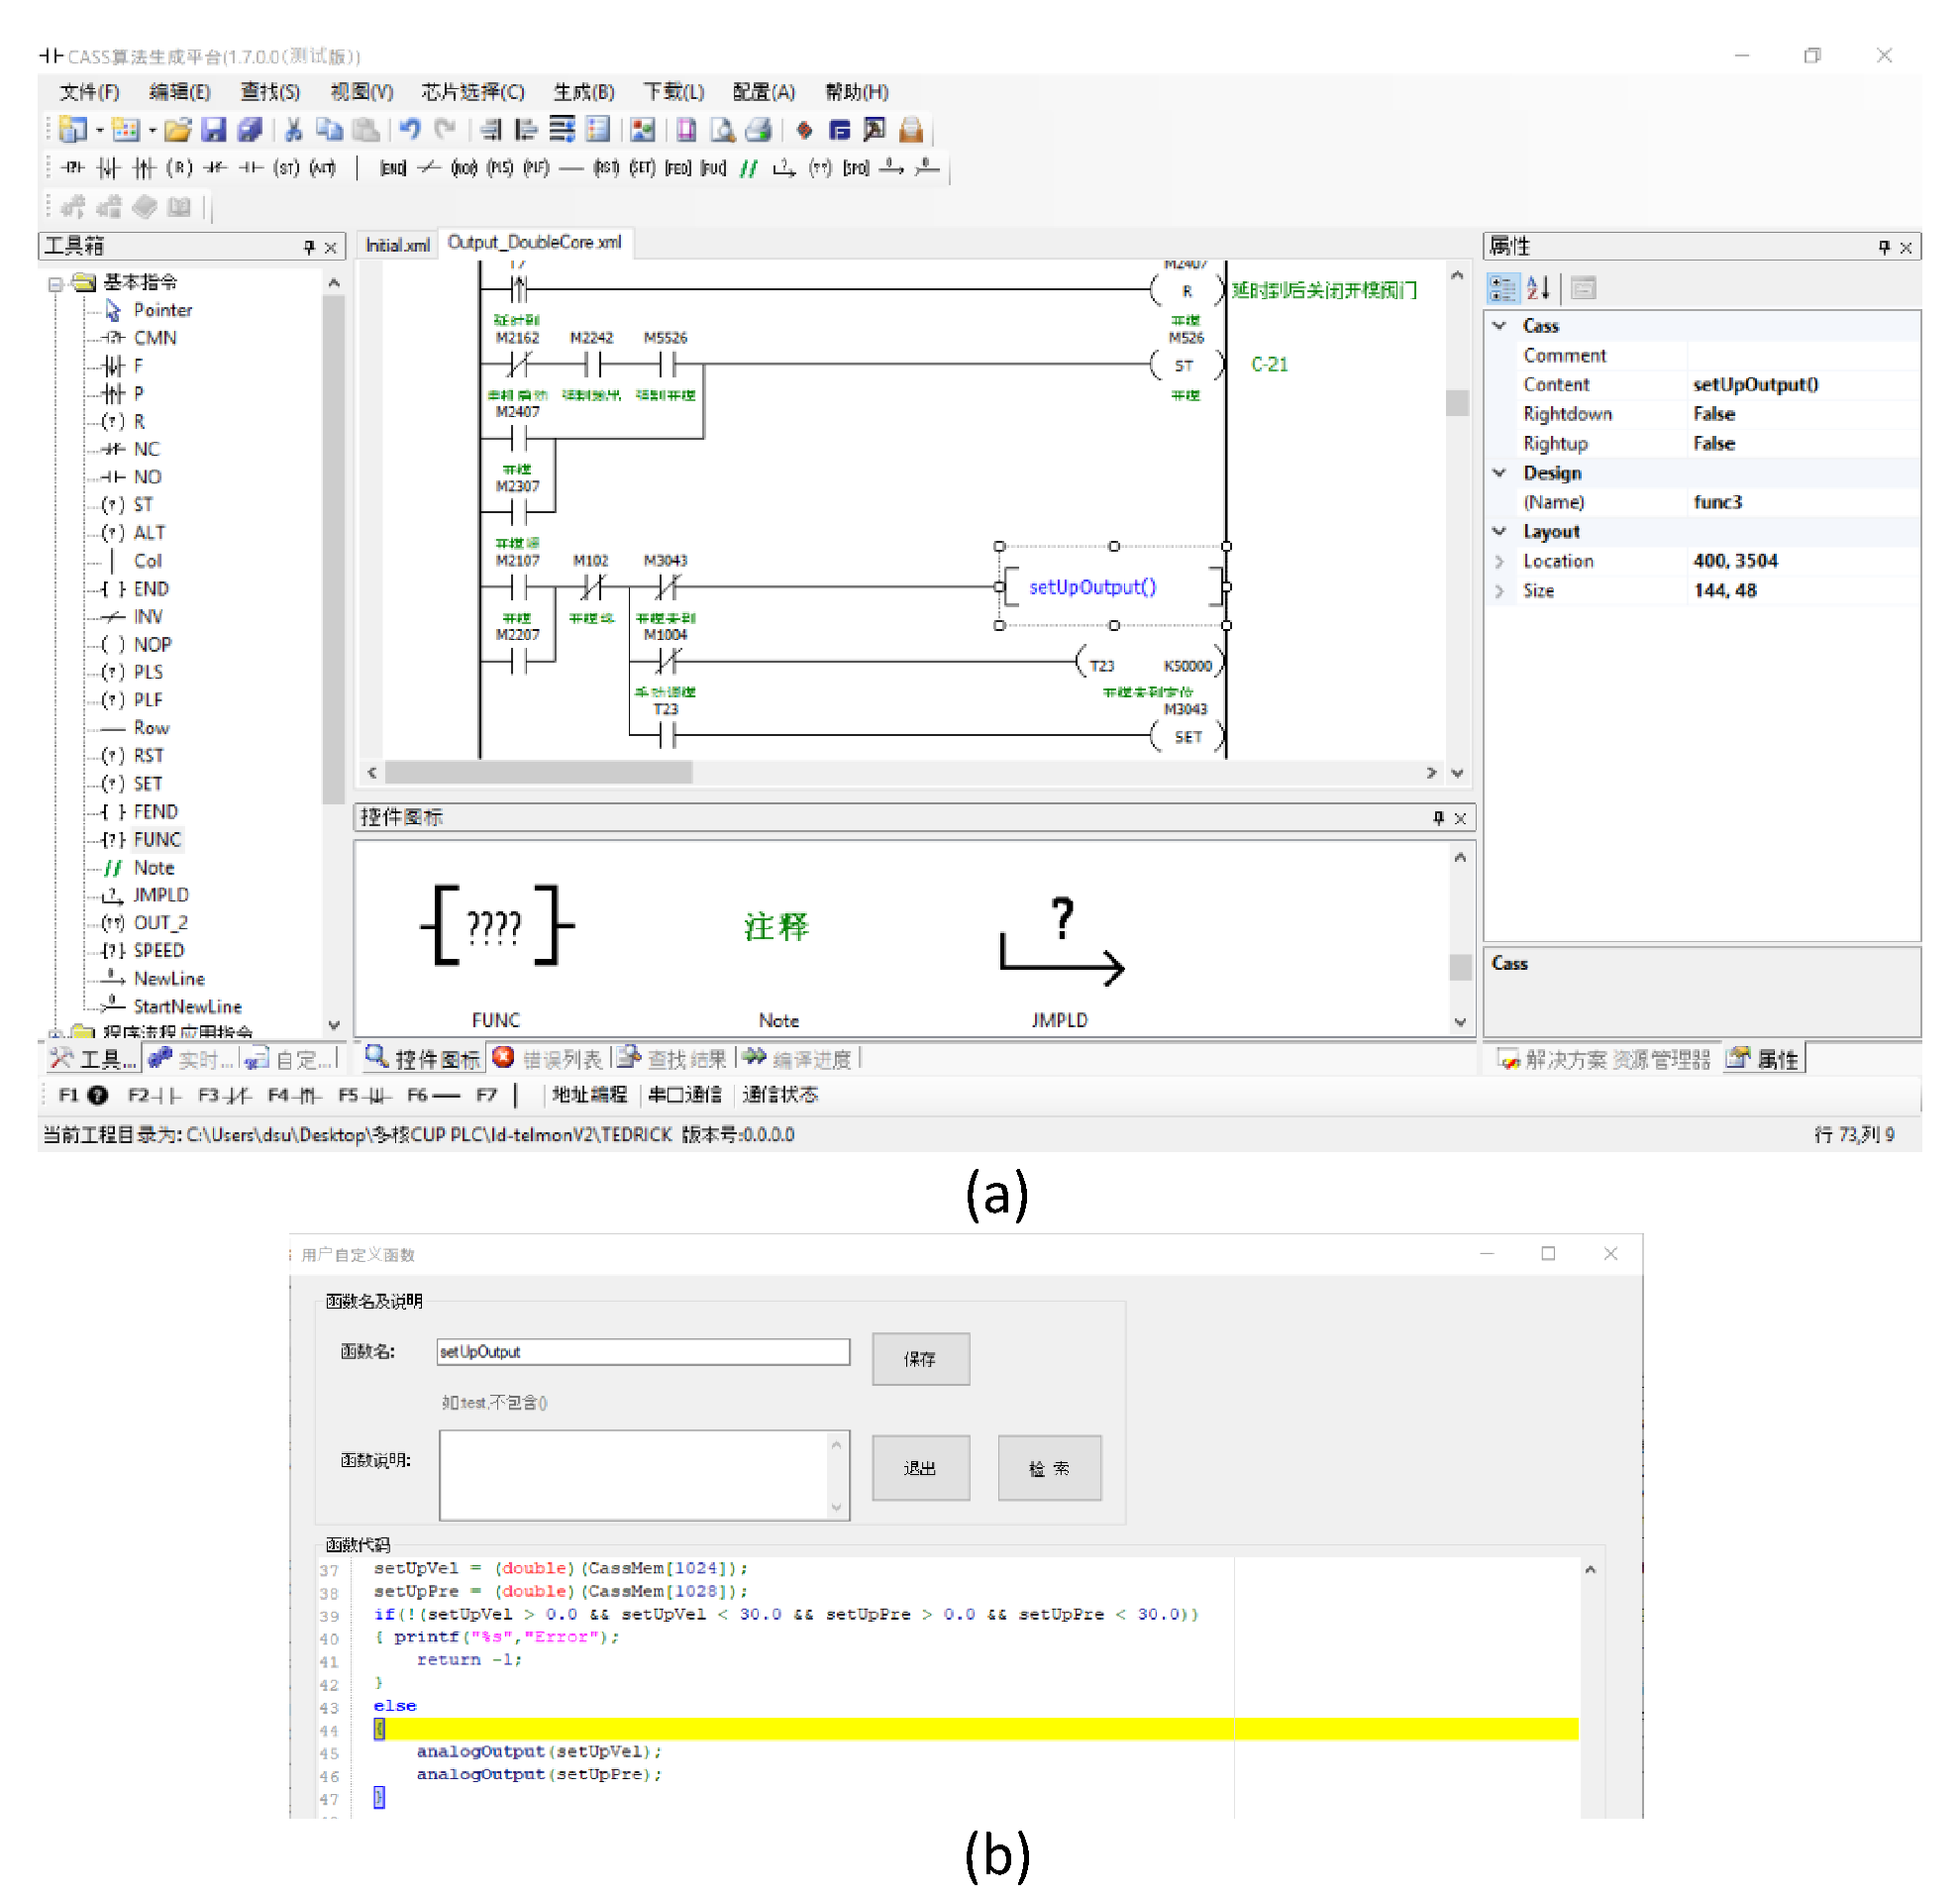
\includegraphics[width=3.5in]{fig/ld.pdf}
	\caption{(a) is the uniform development platform. In the dotted line box, it is the C language component and (b) is its partial code. This component represents to output a small velocity and pressure in setup mode.}
	\label{fig:ld}
\end{figure}

Three typical requirements using the proposed user-oriented development method are discussed below:
\begin{enumerate}
	\item Using multi-processors: adding S-curve acceleration and deceleration algorithm. For this case, we can run the S-curve in the DSP (slave processor).
	\item Design in the uniform development platform: adding an ejector module contained a T-curve. We can design the $LCP$ with $LD$ and the T-curve packaged as a component in the same platform.
	\item Modular Design: inject before high pressure of mold close. Customized a message flag in $MSF$, broadcasting the message when the beginning of high pressure and then the module of injection will get the message and the $CT$ will start it.
\end{enumerate}
\subsection{Analysis}
We compared the system information, development method and key performance among the Techmation system, the KEBA system and the proposed system.

\begin{enumerate}
	\item System information. TECHMATION and KEBA system account for the main market. Due to the reduced complexity, our system can have customized $PLC$ and separated $HMI$. To some extend, it extremely decrease the cost. Our system adopts the widely used distributed structure which decrease wire usage and increase immunity to interference.
	\item Development method. Our system adopted a usr-oriented development method, including customized multiprocessor $ePLC$, component based uniform development platform and comprehensive optimization of the system. Other systems are hard to do these and can not support C language component. Specially, Techmation system is developed by assembly instruction and even do not support IEC61131-3.
	\item Key performance. To our best knowledge, we adopted defective percentage ($DP$), error of change-over position ($EoCP$), error of cushion minimum ($EoCM$), error of charging end position ($EoCEP$) and error of mold open end position ($EoMOEP$) as the key performance. All the systems were adjusted to use T-curve and the key parameters were set the same value. The cycle time, mold close time, mold open time, injection time, charging time and cooling time, ejector forward time and ejector backward time were controlled at about 8 s, 2 s, 2 s, 1 s, 1 s, 1 s, 0.5 s, 0.5 s respectively. Fig. \ref{fig:Compare} shows the 100 times error line graph of the key performance. The proposed system has almost identical performance with KEBA system which is better than TECHMATION system. Talbe \ref{table:IMMSystem} are the comparison of startup time ($ST$), $DP$ and the mean of the key performance. Our system startup time has been increased by more than 20 times in the case of almost identical key performance.
\end{enumerate}
\begin{table}
	\scriptsize \caption{Comparison of System Performance}
	\label{table:ComparisonG}
	\begin{center}
		\renewcommand{\arraystretch}{1.4}
		\setlength\tabcolsep{3pt}
		%\begin{tabular}{|p{2cm}|p{1.5cm}|p{1.5cm}|p{2.3cm}|p{2.3cm}|p{2.3cm}|p{2cm}|}
		\begin{tabular}{|l|c|c|c|c|c|c|}
			\hline
			Brand & ST &DP&mean EoCP&mean EoCM&mean EoCEP&mean EoMOEP\\
			\hline
			Techmation  & 120s  &0.27\% &0.094 & 0.2 & 0.13 & 0.17 \\
			\hline
			KEBA        & 150s  &0.24\% &0.064 & 0.1 & 0.1 & 0.12 \\
			\hline
			Implemented   & 6s     &0.25\% &0.05 & 0.1 & 0.11 & 0.11\\
			\hline
		\end{tabular}
	\end{center}
\end{table}

\begin{figure}
	\centering
	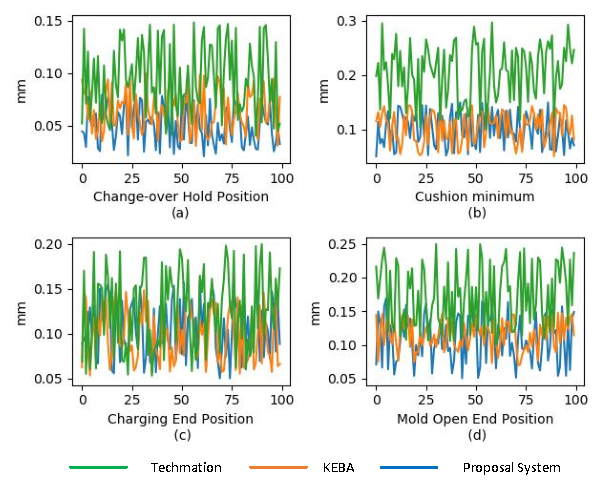
\includegraphics[width=3in]{fig/Compare.pdf}
	\caption{(a) is EoCP, (b) is EoCP, (c) is EoCM, (d) is EoMOEP.}
	\label{fig:Compare}
\end{figure}
\section{Conclusion}
\label{conclusion}
This paper presents a user-oriented development method. We pose the customized mulitprocessor $ePLC$ to enhance the performance, the multi-language supported graphical component to improve the adaptability of developers, the optimized system structure (reasonable memory allocation, user-oriented thread structure, $LPM$ data interaction, modular software design, finite state machines) to reduce the development complexity. Ultimately, we adopt the proposed method to implement the distributed $IMM$ system. By comparison with TECHMATION and KEBA system, our system startup time has been increased by more than 20 times in the case of almost identical key performance and our system support customized multiprocessor $ePLC$ and detached $HMI$.





\ifCLASSOPTIONcaptionsoff
  \newpage
\fi



% trigger a \newpage just before the given reference
% number - used to balance the columns on the last page
% adjust value as needed - may need to be readjusted if
% the document is modified later
%\IEEEtriggeratref{8}
% The "triggered" command can be changed if desired:
%\IEEEtriggercmd{\enlargethispage{-5in}}

% references section

% can use a bibliography generated by BibTeX as a .bbl file
% BibTeX documentation can be easily obtained at:
% http://www.ctan.org/tex-archive/biblio/bibtex/contrib/doc/
% The IEEEtran BibTeX style support page is at:
% http://www.michaelshell.org/tex/ieeetran/bibtex/
%\bibliographystyle{IEEEtran}
% argument is your BibTeX string definitions and bibliography database(s)
%\bibliography{IEEEabrv,../bib/paper}
%
% <OR> manually copy in the resultant .bbl file
% set second argument of \begin to the number of references
% (used to reserve space for the reference number labels box)

\bibliographystyle{IEEEtran}
\bibliography{reference}

% biography section
%
% If you have an EPS/PDF photo (graphicx package needed) extra braces are
% needed around the contents of the optional argument to biography to prevent
% the LaTeX parser from getting confused when it sees the complicated
% \includegraphics command within an optional argument. (You could create
% your own custom macro containing the \includegraphics command to make things
% simpler here.)
%\begin{IEEEbiography}[{\includegraphics[width=1in,height=1.25in,clip,keepaspectratio]{mshell}}]{Michael Shell}
% or if you just want to reserve a space for a photo:

%\begin{IEEEbiography}[{\includegraphics[width=1in,height=1.25in,clip,keepaspectratio]{fig/Author_HuifengWu.eps}}]{Huifeng Wu} received the Ph.D. degree in computer science and technology from Zhejiang university, Hangzhou, China, in 2006. He is currently a professor in the institute of intelligent and software Technology, Hangzhou Dianzi University. His research interests include software development methods and tools, software architecture, embedded system, intelligent control \& automation.
%	
%\end{IEEEbiography}
%\begin{IEEEbiography}[{\includegraphics[width=1in,height=1.25in,clip,keepaspectratio]{fig/Author_YiYan.eps}}]{Yi Yan} received B.S. in automatic control engineering form Zhejiang Sci-Tech University in 1984, M.S. in computer engineering from Beijing University of Postal Telecommunications in 1990. Currently he is the director and full professor in institute of intelligent and software Technology, Hangzhou Dianzi University. His research interests include embedded system, advanced manufacturing system, intelligent control \& automation, and intelligent instruments.
%	
%	
%\end{IEEEbiography}
%\begin{IEEEbiography}[{\includegraphics[width=1in,height=1.25in,clip,keepaspectratio]{fig/Author_DanfengSun.eps}}]{Danfeng Sun} received M.S. in computer architecture from Hangzhou DianZi University in 2011. He is currently a research assistant in the Institute of Industrial Internet, Hangzhou DianZi University. His research interests include embeded system, motion control and IIoT.
%\end{IEEEbiography}
%\begin{IEEEbiography}[{\includegraphics[width=1in,height=1.25in,keepaspectratio,angle=-90]{fig/Author_ReneSimon.eps}}]{Rene Simon} obtained a doctor of engineering at the Otto-von-Guericke University Magdeburg in 2001. He is Professor of Control Systems at the Department of Automation and Computer Sciences, Harz University of Applied Sciences, Wernigerode, Germany. His major research fields include engineering of automation systems, especially industrial controllers. He is chairman of PLCopen and project leader IEC 61131-10 Ed. 1.0.
%\end{IEEEbiography}



% insert where needed to balance the two columns on the last page with
% biographies
%\newpage


% You can push biographies down or up by placing
% a \vfill before or after them. The appropriate
% use of \vfill depends on what kind of text is
% on the last page and whether or not the columns
% are being equalized.

%\vfill

% Can be used to pull up biographies so that the bottom of the last one
% is flush with the other column.
%\enlargethispage{-5in}



% that's all folks
\end{document}


